\documentclass[a4paper,oneside,11pt]{report}

%------------ package pour langue fr ------
\usepackage[utf8]{inputenc}
\usepackage[french]{babel}
\usepackage[T1]{fontenc}
\usepackage{multicol}
\usepackage{enumitem}
\usepackage{multirow}
%------------- for embedding images----------
\usepackage{graphicx} 
\usepackage{float}
\usepackage[export]{adjustbox}
\usepackage{amsfonts,epsfig,epstopdf,titling,url,array}
\usepackage{lscape}

\usepackage{amsmath}
\usepackage{amssymb}
\usepackage{amsthm}
%--------- pour le style de la page ----------
\usepackage[top=3cm, bottom=3cm, left=2.5cm, right=2cm]{geometry}

\usepackage[]{geometry}

\usepackage{algorithm}
\usepackage{algorithmic}


\usepackage{setspace}
\setstretch{1,5}
%\usepackage{txfonts} //pour utiliser times new roman dans le document
\usepackage{fancyhdr}
\pagestyle{fancy}
%\renewcommand\headrulewidth{1pt}
%\fancyhead[L]{Bousbiat Hafsa - Ihadadene Sana}
%\fancyhead[R]{Rapport Master}
%--------------------------- Sommaire ----------------------------%
\usepackage{hyperref}
\usepackage{amssymb}
\usepackage{natbib}
\theoremstyle{definition}
		\newtheorem{defn}{Definition}[section]
		\newtheorem{conj}{Conjecture}[section]
		\newtheorem{exmp}{Example}[section]
\usepackage[table,dvipsnames]{xcolor}	

\usepackage{pifont}% http://ctan.org/pkg/pifont
\newcommand{\xmark}{\color{red}\ding{55}}%
\newcommand{\cmark}{\color{PineGreen}\ding{51}}	
\usepackage[T1]{fontenc}
\newcolumntype{R}[1]{>{\raggedleft\arraybackslash }b{#1}}
\newcolumntype{L}[1]{>{\raggedright\arraybackslash }b{#1}}
\newcolumntype{C}[1]{>{\centering\arraybackslash }b{#1}}


\begin{document}

%Page de garde (page de titre)							Obligatoire

\begin{titlepage}

\newgeometry{top=0mm,right=20mm,left=20mm,bottom=0mm}



	%--------------------  Entete de l'Ecole ----------------------%

	\begin{figure}[t]
		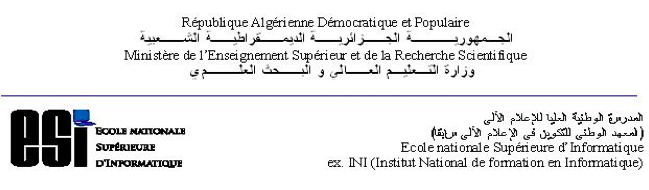
\includegraphics[scale=0.75]{./ressources/image/ESI.png}\\[0.6in]
	\end{figure}
	
	
	
	%--------------------------------------------------------------%
	\begin{center}
	
	%------------------------  Le sujet ---------------------------%
		\LARGE \textbf{ Mémoire}\\
		\Large{
			Pour Obtention du diplôme de Master En Informatique\\
			\textbf{Option : Système Informatique (SIQ)}
			%\textsc thèse D'Ingéniorat En Informatique sous le thème :
		}\\[0.2in]
		\huge {
		\rule{\linewidth}{.5pt}
			\textbf{
				Étude et classification des méthodes de compression de graphe par extraction de motifs et k2-trees
			} 
			\rule{\linewidth}{.5pt}
		}\\[0.5in]
		\Large
	%--------------------------------------------------------------%	
	
	%-------------------------  Mon nom ---------------------------%
	\textbf{Réaliser par:}\\
	\begin{multicols}{2}
			\Large 	Mlle. Hafsa Bousbiat\\
			\large eh\_bousbiat@esi.dz\\
			ESI\\
		\columnbreak
 			\Large Mlle. Sana Ihadadene\\
			\large es\_ihadadene@esi.dz\\
			ESI \\
		
	\end{multicols} 
	
	\vskip 0.1in
	%--------------------------------------------------------------%	

	%-----------------------  Encadreures -------------------------%
	 \textbf{Encadrer par:}\\
	 
	 \begin{multicols}{2}
			\Large 	Dr. Karima Amrouche\\
			\large k\_amrouche@esi.dz\\
			ESI\\
		\columnbreak
 			\Large Dr. Hamida Seba\\
			\large hamida.seba@univ-lyon1.fr\\
			Université de Lyon \\
	\end{multicols}
	
	%--------------------------------------------------------------%	
	
	\small
	\vskip 0.3in
	Octobre 2018 \\
	Année Universitaire: 2018-2019\\
	
	\end{center}		
\restoregeometry
\end{titlepage}

%Remerciements											Obligatoire
\begin{center}
	\par
	\textit{
		\vskip 1in
		\Huge 
			Remerciement \\[0.5in]
			\addcontentsline{toc}{chapter}{\numberline{}Remerciement}
	}
\end{center}
	\par
  Nous tenons d'abord à exprimer notre gratitude à l'égard de nos encadrants, Madame Seba
Hamida, Madame Amrouche Karima et Monsieur Mohammed pour leur précieuse	aide, leur judicieux conseils  et pour le temps qu'ils nous ont consacré tout au long de ce PFE.\\


Nous remercions également toute l'équipe pédagogique de l'École Nationale
Supérieure d'Informatique, et à leur tète les enseignants pour la richesse et la qualité de la formation qu'ils nous ont offert tout au long de notre cursus.\\


Nous tenons à remercier les membres du jury qui nous ont fait l’honneur d’accepter de juger
cet humble travail.\\


Enfin, nous adressons nos plus sincères remerciements à tous nos proches et amis, qui nous ont toujours encouragée au cours de la réalisation de ce mémoire.
Merci à tous et à toutes.

\newpage
 


%Résumé												Obligatoire
\begin{center}
	\par
	\textbf{
		\vskip 0.5in
		\LARGE 
			Résumé \\[0.15in]
			\addcontentsline{toc}{chapter}{\numberline{}Résumé}
	}
\end{center}
	\par
    Lorem ipsum dolor sit, amet consectetur adipisicing elit. Nostrum tempore ea fugiat numquam autem saepe quas porro vitae? Fugit commodi tempore voluptate sint fugiat, possimus optio ad! Pariatur, obcaecati quidem.
Lorem ipsum dolor, sit amet consectetur adipisicing elit. Neque excepturi ducimus accusantium eius voluptatibus, quod velit, explicabo tenetur aliquid ipsam sapiente. Quibusdam quis ullam, saepe numquam molestias nobis recusandae labore?    Lorem ipsum dolor sit, amet consectetur adipisicing elit. Nostrum tempore ea fugiat numquam autem saepe quas porro vitae? Fugit commodi tempore voluptate sint fugiat, possimus optio ad! Pariatur, obcaecati quidem.
Lorem ipsum dolor, sit amet consectetur adipisicing elit. Neque exceptu 

\begin{center}
	\par
	\textbf{
		\vskip 0.5in
		\LARGE 
			Abstract \\[0.15in]
	}
\end{center}
	\par
    Lorem ipsum dolor sit, amet consectetur adipisicing elit. Nostrum tempore ea fugiat numquam autem saepe quas porro vitae? Fugit commodi tempore voluptate sint fugiat, possimus optio ad! Pariatur, obcaecati quidem.
Lorem ipsum dolor, sit amet consectetur adipisicing elit. Neque excepturi ducimus accusantium eius voluptatibus, quod velit, explicabo tenetur aliquid ipsam sapiente. Quibusdam quis ullam, saepe numquam molestias nobis recusandae labore?    Lorem ipsum dolor sit, amet consectetur adipisicing elit. Nostrum tempore ea fugiat numquam autem saepe quas porro vitae? Fugit commodi tempore voluptate sint fugiat, possimus optio ad! Pariatur, obcaecati quidem.
Lorem ipsum dolor, sit amet consectetur adipisicing elit. Neque exceptu

\newpage

%Sommaire (Table des matières)							Obligatoire
\tableofcontents
\newpage

%Liste des figures										Selon besoin
\listoffigures
\addcontentsline{toc}{chapter}{\numberline{}Liste des figures}
\cleardoublepage

%Liste des tableaux										Selon besoin

\listoftables
\addcontentsline{toc}{chapter}{\numberline{}Liste des tableaux}
\cleardoublepage

%Introduction (début de la pagination)					bligatoire


\chapter{Introduction} 


%---->chapitre 01 :« cadrage du projet »
	\chapter{ Théorie des graphes}
	  Pour faciliter la compréhension d'un problème, nous avons tendance à  le dessiner ce qui nous amène parfois même à le résoudre. La théorie des graphes est fondée à l'origine sur ce principe. De nombreuses propriétés et méthodes ont été pensées ou trouvées à partir d'une représentation schématique pour être ensuite formalisées et prouvées.


La théorie des graphes est historiquement un domaine mathématique qui s'est développé  au sein des autres disciplines comme la chimie, la biologie, la sociologie et l'industrie. Elle constitue aujourd'hui un corpus de connaissance très important et un instrument efficace pour résoudre une multitude de problèmes.


De manière générale, le graphe sert à représenter les structures, les connexions entre différents composants, les acheminements possibles pour un ensemble complexe composé d'un grand nombre de situations en exprimant les dépendances et les relations entre ses éléments,(e.g. réseau routier ou ferroviaire, réseau de communication, diagramme d'ordonnancement, ..). 


Dans ce chapitre, nous présenterons les notions et les concepts clés relatives aux graphes qui serviront de base pour la suite de notre travaille, à savoir : la définition d'un graphe, ses types et sa représentation structurelle. Nous clôturons le chapitres avec quelques domaines d'application des graphes.

	
	\section{Graphe non orienté}
			\subsection{Définitions et généralités}
		
Un graphe non orienté G est la donnée d’un couple (V , E) où V = \{$ \textit{v}_{1} , \textit{v}_{2} ,..., \textit{v}_{n} $\} est un ensemble fini dont les éléments sont appelés sommets ou nœuds ( Vertices en anglais ) et  E=\{$\textit{e}_{1} ,  \textit{e}_{2} ,…, \textit{e}_{m} $\} est un ensemble fini d'arêtes ( Edges en anglais ). Toute arête \textit{e} de E correspond à un couple non ordonné de sommets ( $\textit{v}_{i} , \textit{v}_{j}$ ) $\in$ E $\subset$  $V \times V$ représentant ses extrémités \citep{muller} \citep{fages2014exploitation}.
\\Soient \textit{e} = ($\textit{v}_{i} , \textit{v}_{j}$) et \textit{e'}=($\textit{v}_{k} , \textit{v}_{l}$) deux arêtes de E, On dit que :
\begin{itemize}
\item $\textit{v}_{i}$ et $\textit{v}_{j}$ sont les extrémités de \textit{e} et \textit{e} est incidente à $\textit{v}_{i}$ et $\textit{v}_{j}$ \citep{hennecart2012elements}.
\item $\textit{v}_{i}$ et $\textit{v}_{j}$ sont voisins ou adjacents, s'il y a au moins une arête entre eux dans E \citep{IUTLyonInformatique}.
\item L'ensemble des sommets adjacents aux deux extrémités de \textit{e} est appelé le voisinage de \textit{e} \citep{muller}. 
\item \textit{e} et \textit{e'} sont voisins s'ils ont une extrémité commune  \citep{lopez2003cours}.
\item L'arête \textit{e} est une boucle si ses extrémités coïncident, i.e, $\textit{v}_{i}$ = $\textit{v}_{j}$ \citep{IUTLyonInformatique}. 
\item L'arête \textit{e} est multiple si elle a plus d'une seule occurrence dans l'ensemble E.
\end{itemize}	
		 
\subsection{Représentation graphique}
Un graphe non orienté G peut être représenté par un dessin sur un plan comme suit \citep{muller}:

\begin{itemize}
\item Les nœuds $\textit{v}_{i}$ $\in$ V de G sont représentés par des points distincts.
\item 	Les arêtes \textit{e} = ($\textit{v}_{i}$,$\textit{v}_{j}$) $\in$ E de G sont représentés par des lignes, pas forcement rectilignes, qui relient les extrémités de chaque arête \textit{e}.
\end{itemize}

%% L'exemple de la représentation graphique 
\textbf{Exemple :}
 Soit g=(V1 , E1) un graphe non orienté tel que : V1=\{ 1,2,3,4,5 \} et E1=\{(1,2), (1,4), (2,2), (2,3), (2,5), (3,4)\}.
La représentation graphique de g est alors donnée par le schéma de la figure \ref{graphNonOriente}.
\\
\begin{figure}[H]
\begin{center}
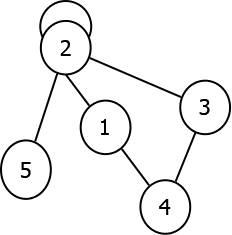
\includegraphics[height=120 pt, width=130 pt]{./ressources/image/graphNonOriente.png} 
\end{center}
\caption{Exemple de représentation graphique d'un graphe non orienté}
\label{graphNonOriente}
\end{figure}

		\subsection{Propriétés d'un graphe}
		
		\begin{itemize}[label=$\circ$]
			
			\item \textbf{Ordre d'un graphe:} On appelle ordre d’un 					graphe le nombre de ses sommets, i.e, Card(V) \citep{DUT}.
			
			\item  \textbf{Taille d'un graphe:} On appelle taille d’un 				graphe le nombre de ses arêtes, i.e, Card(E) \citep{DUT}.
			
			\item  \textbf{Degré dans un graphe:}
			
			
			\begin{itemize}[label=$\bullet$]
				\item \textbf{Degré d'un sommet : } Le degré d’un sommet noté \textit{d}($\textit{v}_{i}$) est le nombre d'arêtes incidentes à ce sommet, sachant qu’une boucle compte pour deux \citep{muller}. Dans l'exemple de la figure \ref{graphNonOriente}, le degré du sommet (1) est : \textit{d}(1)=2.
				
				\item \textbf{Degré d'un graphe : }Le degré d’un graphe est le degré maximum de ses sommets, i.e, max(\textit{d}($\textit{v}_{i}$)) \citep{muller}. Dans l’exemple de 				la figure \ref{graphNonOriente}, le degré du graphe g est \textit{d}(2)=5.
			\end{itemize}
			
			\item \textbf{Rayon et diamètre dans un graphe:}
			\begin{itemize}[label=$\bullet$]
				\item \textbf{Distance : }La distance entre deux sommets 	\textit{v} et \textit{u} est le plus petit nombre d’arêtes qu’on doit parcourir pour aller de \textit{v} à \textit{u} ou de \textit{u} à \textit{v} \citep{muller}. 
				
				\item 	\textbf{Diamètre d’un graphe :} C’est la plus grande 	distance entre deux sommets de ce graphe \citep{muller}. 
				
				\item 	\textbf{Rayon d’un graphe : }C’est la plus petite distance entre deux sommets de ce graphe \citep{parlebas1972centralite}. 
			\end{itemize}
		\end{itemize}
		
	
			
	
			
	\section{Graphe orienté}	
		
		\subsection{Définitions et généralités}
		Un graphe orienté G est la donnée d'un couple (V , E) où
		V est un ensemble fini dont les éléments sont appelés les sommets de G et 
		E  $\subset$ V x V est un ensemble de couples ordonnés de sommets dits arcs ou arêtes \citep{muller}. G est appelé dans ce cas digraphe (directed graph).\\
		 Pour tout arc e = ( $v_{i}$ , $v_{j}$) $\in$ E :
		 \begin{itemize}  
			\item $v_{i}$ est dit extrémité initiale ou origine de e et $v_{j}$ est l'extrémité finale de e \citep{muller}.
			
			\item $v_{i}$ est le prédécesseur de $v_{j}$ et $v_{j}$ est le successeur de $v_{i}$ \citep{IUTLyonInformatique}.
			
			\item les sommets $v_{i}$ , $v_{j}$ sont des sommets adjacents \citep{Pres}.
			
			\item e est dit sortant en $v_{i}$ et incident en $v_{j}$ \citep{Pres}.
			
			\item e est appelé boucle si $v_{i}$ = $v_{j}$, i.e l'extrémité initiale et finale représente le même sommet \citep{IUTLyonInformatique}.
			
		\end{itemize}
		 
		
		\subsection{Représentation graphique}
		
		
		Un graphe G = (V , E) peut être projeter sur le plan en représentant:
		\begin{itemize} 
		\item Dans un premier temps les nœuds $v_{i}$ $\in$ V par des points disjoints du plan.
		\item Et dans un second temps les arêtes e = ( $v_{i}$ , $v_{j}$) $\in$ E par des lignes orientées reliant par des flèches les deux extrémités de e. 
		\end{itemize}
		
		\textbf{Exemple:}
		
		Soit g = ($V_{1}$ , $E_{1}$) un digraphe tel que : $V_{1}$ = \{ 1,2,3,4 \} et  $E_{1}$ = \{(1,2),(1,3),(3,2),(3,4),(4,3)\}.
		
		Le représentation graphique de g est alors donné par le schéma de la figure \ref{grapheOr}.
	
		
			\begin{figure}[h]
			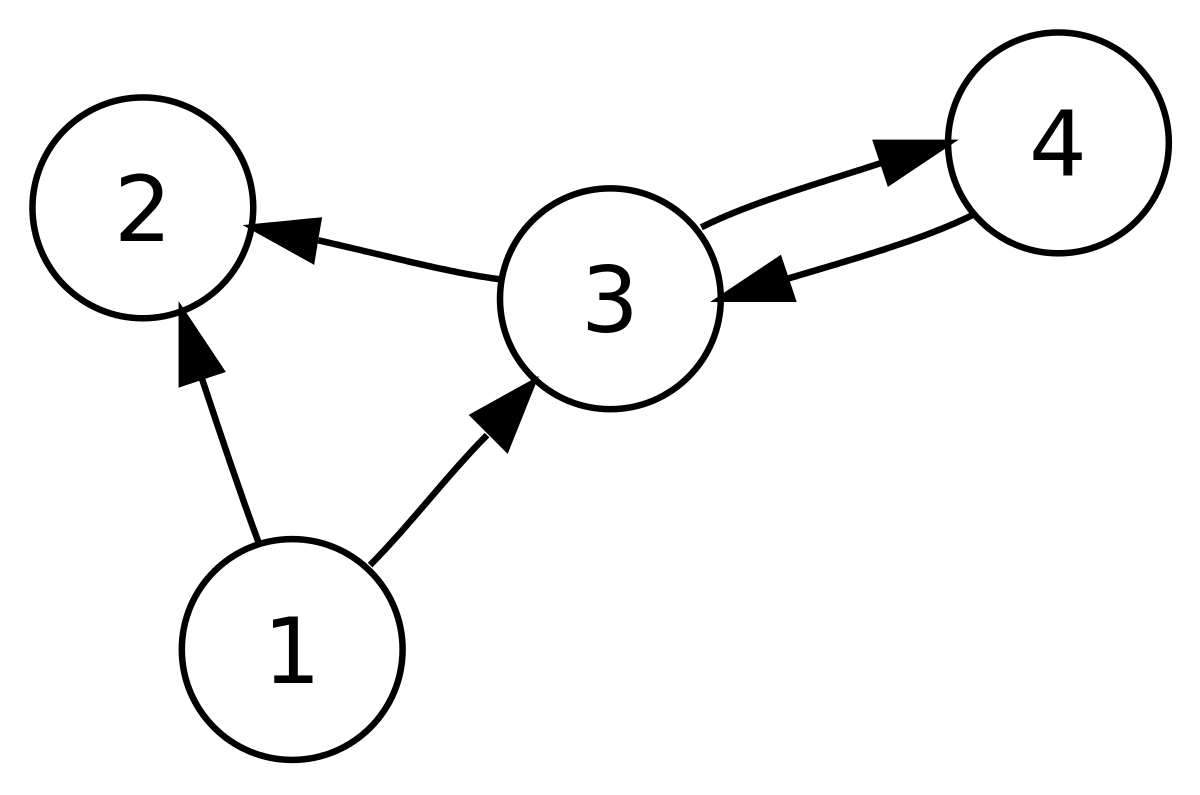
\includegraphics[scale=0.15,center]{./ressources/image/RepDiGraphe.png}
			\caption[Exemple de représentation graphique d'un digraphe.]{Exemple de représentation graphique d'un digraphe.}
			\label{grapheOr}
			\end{figure}
			
		
		\subsection{Quelques Propriétés:} %%% Arevoire 
			\begin{itemize}[label=$\circ$]
			\item\textbf{Ordre d'un digraphe:}
			est le nombre de sommets n = Card(V) \citep{DUT}.
			
			\item\textbf{taille d'un digraphe:} est le nombre d’arcs m = Card(A) \citep{DUT}.
			
			\item\textbf{Degré dans un digraphe:}
			Le degré d'un sommet $v_{i}$ $\in$ V dans un digraphe G=(V , E) est donnée par la formule :
			\begin{center}
				d($v_{i}$) = $d^+(v_{i}$) + $d^-(v_{i}$\\
			\end{center}			 
			 où $d^+(v_{i}$) est le nombre d'arcs sortants au sommet $v_{i}$ et est appelé degré extérieure et $d^-(v_{i}$) représente le nombre d'arcs incidents et est appelé degré intérieur \citep{muller}.
			 
			 \item\textbf{Voisinage dans un digraphe:}
			 Le voisinage d'un sommet $v_{i}$ $\in$ V, noté V($v_{i}$), dans un digraphe G = (V , E) est:
			 	\begin{center}
				V($v_{i}$) = succ($v_{i}$) $\bigcup$ pred($v_{i}$),
				\end{center}
				
				où succ($v_{i}$) est l'ensemble des successeurs de $v_{i}$ et pred($v_{i}$) est l'ensemble de ses prédécesseurs \citep{bac}, i.e le voisinage de $v_{i}$ est l'ensemble des sommets qui lui sont adjacents.
			
			\end{itemize}
			
		
	\section{Notion de Connexité}
	
	Les structures de graphes sont généralement exploitables à travers leurs interrogation qui permet de fournir des réponses aux problèmes modélisés. L'un des informations les plus importantes dans un graphe est la notion des relations (indirectes ou indirecte) entre deux nœuds ou plus formellement la connexité dans un graphe. Dans cette partie nous allons définir les concepts relatives à cette notion.
	
	\begin{itemize} [label = $\bullet$]
		
			 
			 \item \textbf{Chemin (resp. Chaine):}
			est une liste de sommets S= $(v_{0},v_{1},v_{2},...,v_{k})$ telle qu’il existe un arc (resp. une arête) entre chaque couple de sommets successifs.
			 
			 
			  \item \textbf{Cycle (resp. Circuit):} 
			 est un chemin (resp. chaine) dont le premier et le dernier sommet sont identiques \citep{DUT}.
			 
			 		\item \textbf{Graphe connexe:}
			Un graphe non orienté (resp. orienté) est dit connexe (resp. fortement connexe) si pour tout pair de sommets ($v_{i}$, $v_{j}$) il existe un chemin S les reliant \citep{muller}.
			 
		\end{itemize}
	
	
	
	\section{Graphe partiel et sous graphe:}
    		
	La quantité de données disponible aujourd'hui et sa croissance de manière exponentielle ont favorisé la décomposition des graphes en des entités plus petites afin de garantir une facilité de compréhension et d'analyse dans le but d'extraire l'information la plus pertinente. Dans cette partie, nous allons définir de manière plus formelle ce que ces entités sont, ainsi que leurs types.
	
		
		
		
		\subsection{Définitions:}
		Soient G = (V , E), $G' = (V' , E')$ et $G'' = (V'' , E'')$ trois graphes.
		\begin{itemize}[label=$\circ$]
		
			\item Le graphe $G'$ est appelé \textbf{graphe partiel} de G si : $V' = V\ et\ E' \subset$ E \citep{DUT}. En d'autres termes, un graphe partiel est obtenu en supprimant une ou plusieurs arêtes de G.
				

			\item Le graphe $G''$ est dit \textbf{sous-graphe} de G si: $V''\subset V$ et 
			 $E''\subset E \cap (V'' x V'')$ \citep{bac}, i.e, un sous-graphe est obtenu en enlevant un ou plusieurs nœuds du graphe initial ainsi que les arêtes dont ils représentent l'une des deux extrémités.
			 
		\end{itemize}
		
		\subsection{Quelques Types de sous graphes:}
		
		\begin{itemize} [label = $\bullet$]
		
		
			\item \textbf{Une Clique :} est un sous-graphe complet de G \citep{bac}.
			
			\item \textbf{Biparti :} G' est un sous-graphe biparti si il existe une partition de V' en deux sous ensembles notés $V_{1}$ et $V_{2}$, i.e V' = $V_{1} \cup V_{2}$ et $V_{1}$ $\cap$ $V_{2}$ = $\phi$, tel que E' = $V_{1}$ x $V_{2}$ \citep{bac}.
			
			\item \textbf{Étoile :}
			 est un cas particulier de sous-graphe biparti où $V_{1}$ est un ensemble contenant le sommet central (dit \textit{hub}) uniquement et $V_{2}$ contient le reste des nœuds  (dits \textit{spokes})\citep{koutra2015summarizing} .
			 
		
			 
		\end{itemize}		
	
	\section{Quelques types de graphe}
		 %% classifier selon le type du graphe en entree
	Avec les avancées technologiques au fil du temps, plusieurs types de graphes ont connus le jours. En effet, La complexité et la variété des problèmes scientifiques existants modélisés par ces derniers ont poussé les chercheurs à adapter leurs structure selon le problème auquel ils font face. Durant cette section nous allons définir les principaux types existants.
	
		\begin{itemize}[label=$\circ$]
		
			\item \textbf{Graphe Complet:} Un graphe G = (V , E) est un graphe complet si tous les sommets $v_{i}$ $\in$ V sont adjacents \citep{Pres}. Il est souvent noté $K_{n}$ où n = card(V) \citep{DUT}.
				
			
			\item \textbf{Graphe étiqueté et graphe pondéré:}
			 Un graphe étiqueté G = (V , E , W) est un graphe, qui peut être orienté ou non orienté, dont chacune des arêtes $e_{i}$ $\in$ E est doté d'une étiquette $w_{i}$. Si de plus, $w_{i}$ est un nombre alors G est dit graphe pondéré (valué) \citep{DUT}.
		
			\item \textbf{Graphe simple et graphe multiple:}
			Un graphe G = (V , E) est dit simple si il ne contient pas de boucles et toute paire de sommets est reliée par au plus une arête. Dans le cas contraire, G est dit multiple \citep{IUTLyonInformatique}.
			
		
		\end{itemize}
			
	
	
    		
    	\section{Représentation Structurelle d'un graphe}	
		\input{./Chapitres/TheorieDesGraphes/structRep.tex}
	
	\section{Les domaines d'application}
		  La diversité des domaines faisant appel à la modélisation par des graphes ne cesse d'augmenter, allant des réseaux sociaux aux réseaux électriques et réseaux biologiques et arrivant jusqu'aux World Wide Web. Dans cette partie nous allons décrire trois domaines d'application les plus répandus des graphes.
	
		\subsection{Graphes des réseaux sociaux:}
		Les réseaux sociaux représentent un lieu d'échange et de rencontre entre individus (entités) et dont l'utilisation est devenue de nos jours une nécessité.  
		Pour représenter les interactions entre ces individus, nous avons généralement besoin de faire recours aux graphes où les sommets sont des individus ou des entités et les interactions entre eux sont représenté par des liens. 
		Vue la diversité des interactions sociales, la modélisation de ces réseaux  nécessite différents types de graphes: graphes non orientés pour pour les réseaux sociaux avec des relations non
orientées, graphes orientés pour représenter des relations non symétriques
comme c'est la cas dans les réseaux de confiance, graphes pondérés pour les réseaux sociaux qui contiennent différents niveaux d'intensités dans les relations, ... etc \citep{lemmouchi2012etude}.
		
		\subsection{Graphes en Bioinformatique:}
		
		La bio-informatique est un domaine qui se trouve à l'intersection des deux grands domaines celui de l'informatique et celui de la biologie. Elle a pour but d'exploiter la puissance de calcule des équipements informatiques pour effectuer des traitements sur des données moléculaires massives \citep{pellegrini2004protein}.
		
		Elle est largement utilisée pour l’analyse des séquences d’ADN et des protéines à travers leurs modélisation sous forme de graphe. A titre d'exemple, les graphes non orientés multiples sont un outil modélisation des réseaux d’interaction protéine-protéine \citep{pellegrini2004protein}, 
		le but dans ce cas est donc l'étude du fonctionnement des protéines par rapport à d'autre.
		
		\subsection{Le Graphe du web:}
		 Le graphe du Web est un graphe orienté dont les sommets sont les pages du web et les arêtes modélise l'existence d'un lien hypertexte dans une page vers une autre \citep{brisaboa2009k}. Il représente l'un des graphes les plus volumineux: en juillet 2000 déja, on estimait qu’il contenait environ 2,1 milliards de sommets et 15 milliards d’arêtes avec 7,3 millions de pages ajoutées chaque jour \citep{guillaume2002web}. De ce fait, ce graphe a toujours attiré l'attention des chercheurs. En effet, l'étude de ses caractéristiques a donné naissance à plusieurs algorithmes intéressants, notamment l'algorithme PageRank de classement des pages web qui se trouve derrière le moteur de recherche le plus connu de nos jours : Google.	
		
	
	
			
	\section{Conclusion}
Dans ce chapitre nous avons présenter les notions et les concepts généraux qui touchent à la théorie de graphes : définitions de graphes, leurs principales propriétés, leurs représentations ainsi que leurs domaines d'application.\\
Le point important qu'on a put tirer de cette partie est que les graphes sont devenue un moyen crucial et indispensable dans la modélisation des problèmes dans plusieurs domaines. Cependant ils deviennent de plus en plus complexes et volumineux avec la grande quantité de données disponible de nos jours, ce qui rend leurs stockage, visualisation et traitement difficile. La compression de graphe est naît comme solution à ce problème. Dans le chapitre suivant nous allons présenter la compression de graphes, son rôle et ses différents méthodes.  
	
	
	

%---->chapitre 02 :« »
	\chapter{Compression de graphe}
	
		\section{Compression de données: }
			 La compression de données est principalement une branche de la théorie de l'information  qui traite des techniques et méthodes liées à la minimisation de la quantité de données à transmettre et à stocker.
Sa caractéristique de base est de convertir une chaîne de caractères vers un autre jeu de caractères occupant un espace mémoire le plus réduit possible tout en conservant le sens et la pertinence de l'information \citep{lelewer1987data}.

	Les techniques de compression de données sont principalement motivées par la nécessité d'améliorer l'efficacité du traitement de l'information. En effet, la compression des données en tant que moyen peut rendre l'utilisation des ressources existantes beaucoup plus efficace. 
	
	De ce fait, une large gamme d'applications usant de ce domaine tel que le domaine des télécommunications et le domaine du multimédia est apparue offrant une panoplie d'algorithmes de compression \citep{sethi2014data}. Sans les techniques de compression, Internet, la télévision numérique, les communications mobiles et les communications vidéo, qui ne cessaient de croître, n'auraient été que des développements théoriques.
	
	%Afin de pouvoir comparer entre ces différentes méthodes de compression, plusieurs critères ont été proposés dans la littérature. Parmi les mesures utilisées on trouve:
	%\begin{itemize}
	%	\item \textbf{Le taux de compression:} représente le rapport entre la taille des données après et avant la compression.
		
		%%% donner la formule
		
		%\item \textbf{Le facteur de compression:} représente l'inverse du taux de compression.
		
		%\item \textbf{Le temps de compression:}
	%\end{itemize}
			
		
		\section{Compression appliquée aux graphes:}
	
			\subsection{Motivations derrière la compression de graphes: }
	
			\subsection{Les types de compression:}
			La compression de graphe est définie comme l'ensemble des méthodes et techniques permettant de réduire l'espace mémoire occupé par ce derniers sans perte significative d'information. Dès lors, deux approches se présente: la compression avec ou sans perte, que nous allons détaillées dans ce qui suit.
			
			\subsubsection{Compression Sans Perte:}
			Certains domaines d'application de la compression nécessitent un niveau élevé d'exactitude et une restitution exacte, donc une compression sans perte. Dans cette catégorie, le graphe G subi des transformation pour avoir une représentation compacte G' qui lors de la décompression donne exactement G. La figure ci-dessous illustre cette définition. 
			
			\begin{figure}[h]
			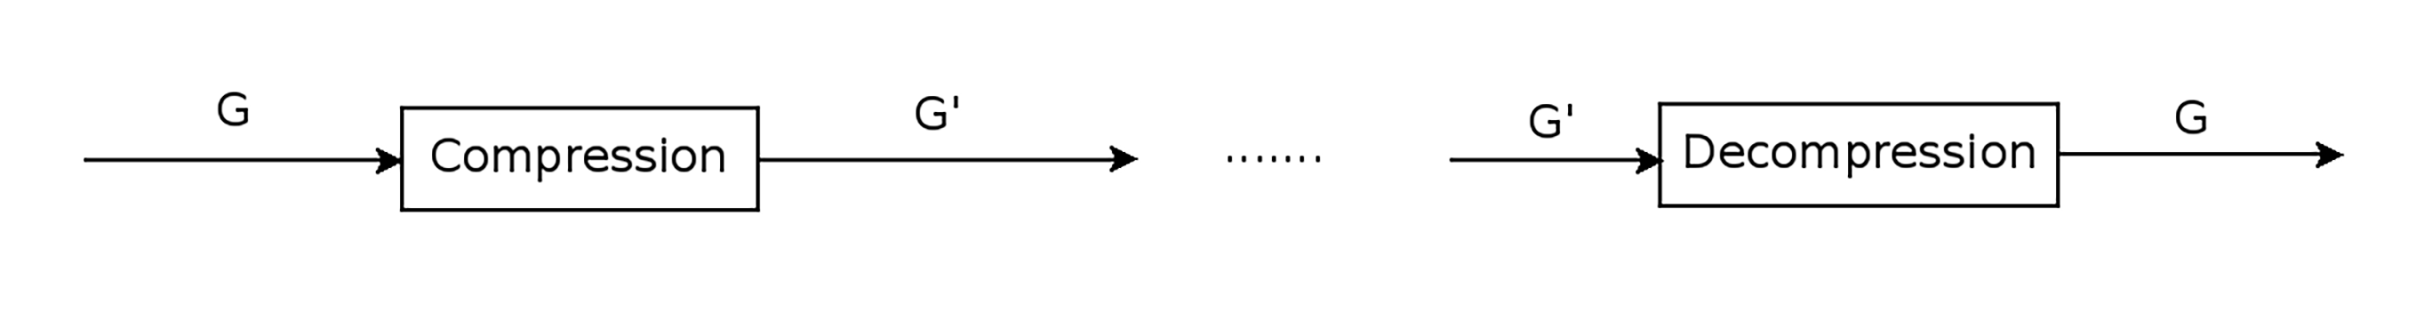
\includegraphics[scale=0.15,center]{./ressources/image/SansPerte.png}
			\caption[Compression sans perte.]{Compression sans perte.}
			\end{figure}
			
			%% citee qlq exemple de compression sans pertes
			
			\subsubsection{Compression Avec Perte:}
			Contrairement à la compression sans perte, la compression avec perte permet la suppression permanente de certaines informations jugées inutile (redondantes) pour améliorer la qualité de la compression.  En d'autres termes, le graphe G subi des transformations pour avoir une représentation compacte G' qui lors de la décompression donne un graphe G'' probablement différent de G mais l'approximant le plus possible. La figure ci-dessous illustre cette définition.   
			
			\begin{figure}[h]
			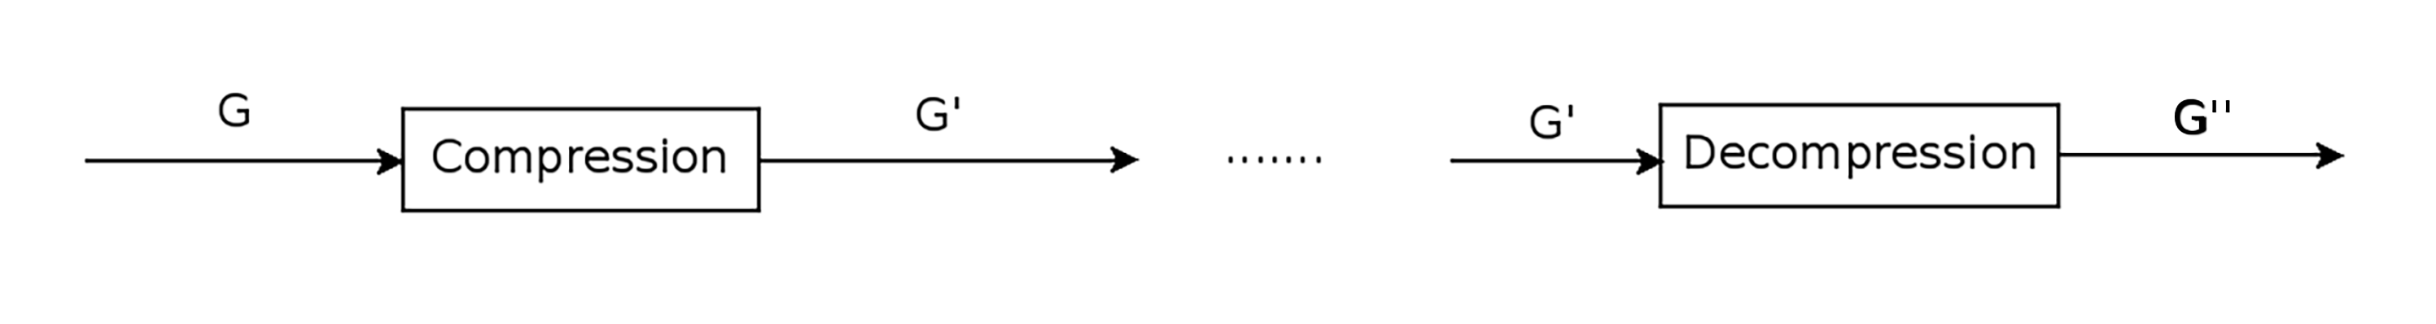
\includegraphics[scale=0.15,center]{./ressources/image/AvecPerte.png}
			\caption[Compression avec perte.]{Compression avec perte.}
			\end{figure}
			
			%%% citee qlq exemple de compression avec perte
			
	
			\subsection{Les métriques d'évaluation des algorithmes de compression:}
					
				Devant la panoplie d'algorithmes et de techniques de compression de graphe disponibles dans la littérature, des critères de comparaison  et d'évaluation entre ces méthodes doivent être bien définis. Dans cette partie nous présenterons les principaux mesures de performances.
				
				\subsubsection{Le temps de compression:}
				C'est une métrique qui donne le temps d'exécution de l'algorithme de compression. Elle est généralement mesurée en secondes (ou ms).
				\subsubsection{Le ratio de compression:}
				C'est la mesure la plus courante pour calculer l'efficacité d'un algorithme de compression. Il est défini comme le rapport entre le nombre total de bits requis pour stocker des données non compressées et le nombre total de bits nécessaires pour stocker des données compressées.
				%la formule
				\begin{center}
				$
				CR = \frac{No.\ de\ bits\ du\ graphe\ originale}{No.\ de\ bits\ du\ graphe\ finale }
				$
				\end{center}
				
				
				Le CR est parfois appelé bit par bit (bpb) et il est définit alors comme étant le nombre moyen de bits requis pour stocker les données compressées \citep{uthayakumar2018survey}. Dans le cas des algorithmes de compression de graphe on a:
				\begin{itemize}
					\item \textbf{Le nombre de bits par nœuds:}
					représente l'espace mémoire nécessaire pour stocker un nœud (bpn pour bits per node).
					%% la formule
					
					\item \textbf{Le nombre de bits par liens:}
					représente l'espace mémoire nécessaire pour stocker un liens (bpe pour bits per edge).
					%%la formule 
				\end{itemize}
				
				
				
				
				
				
				\subsubsection{Le taux de compression:}
				Exprimée en pourcentage, cette métrique permet de mesurer la performance de la méthode de compression. Elle peut être exprimer de deux manières différentes:
				
				\begin{itemize}
					\item \textbf{Le taux de compression:} Le rapport entre volume du graphe après compression et le volume initial du graphe.
					\begin{center}
				$
				t = \frac{La\ taille\ du\ graphe\ finale}{La\ taille\ du\ graphe\ originale }
				$
				\end{center}
					\item \textbf{Le gain d'espace: }Le gain d'espace représente la réduction de la taille du graphe compressé par rapport à la taille du graphe original.
					
					\begin{center}
				$
				G = 1 - \frac{La\ taille\ du\ graphe\ finale}{La\ taille\ du\ graphe\ originale }
				$
				\end{center}
					
					
				\end{itemize}
				
				
				%\subsubsection{L'erreur quadratique:}
			
			\subsection{Classification des méthodes de compression:}
				Le domaine de compression des graphes est un domaine qui a connu une grande évolution vu son importance. Une multitude de méthodes ont été proposées au cours des dernières années. Elles diffèrent l'une de l'autre dans plusieurs points : le type de graphe en entrée, le type de structure en sortie, le type de compression et la technique utilisée pour la compression. En se basant sur ces différences, plusieurs classifications ont été suggérées. Nous allons dans ce qui suit présenter les plus importantes parmi ces classifications.\\

Dans \citep{maneth2015survey}, les auteurs proposent une classification basée tout d'abords sur le type de compression. Ils regroupent les méthodes en deux catégories principales : les méthodes de compression sans perte et les méthodes de compression avec perte. La première catégorie est subdivisée à son tour selon le type de représentation du graphe en sortie : représentation succinte, représentation structurelle ou une représentation sous forme de fichier RDF\newacronym{rdf}{RDF}{Resource Description Framework}\footnote{\gls{rdf} : est un modèle de graphe destiné à décrire de façon formelle les ressources Web et leurs métadonnées, de façon à permettre le traitement automatique de telles descriptions.}. 
Les méthodes donnant une représentation succincte représentent le graphe sous forme d'une chaine de bits succincte irréversible lors de la décompression. La sortie de ces méthodes est ainsi une structure compacte du graphe originale. Parmi les méthodes de cette classe, nous trouvons : Web Framework de Boldi et Vigna \citep{boldi2004webgraph}. La deuxième classe est la représentation structurelle. Contrairement à l'approche précédente, les méthodes de cette classe modifient la structure du graphe initial, sachant que les modifications apportées sont réversibles. La sortie sera donc une structure réduite et non pas compacte de la version initiale. Parmi ces méthodes, nous citons : RePair de Claude et Navarro \citep{claude2010fast}. La dernière classe est la compression  des fichiers \gls{rdf} et qui comporte des méthodes assez récente. Nous trouvons parmi ces techniques : Dcomp de \citep{martinez2012compression} . Les méthodes de compression avec perte quant à elles apportent des modifications irréversibles sur le graphe en supprimant les informations redondantes et le bruit. Comme exemple, nous citons : ASSG de Zhang et al. \citep{zhang2014assg}.\\

Une autre classification a été exposée par Lui et al. dans \citep{liu2018graph} qui classe les méthodes sur trois niveaux. Au premier et deuxième niveaux, les techniques de compression sont regroupées en fonction du type de graphe en entrée selon deux critères : graphe statique ou dynamique et graphe simple ou étiqueté. Pour le troisième niveau, les auteurs catégorisent les méthodes selon la technique de traitement utilisée. Quatre catégories sont définies: les méthodes de regroupement ou d'agrégation, ces méthodes permettent d'agréger de manière récursive un ensemble de nœuds, liens ou carrément un cluster en un super nœud (appelé parfois nœud virtuel), comme exemple de ces techniques, nous trouvons Grass \citep{lefevre2010grass}. Le deuxième type de méthodes englobe les méthodes de compression de bits. Ces méthodes minimisent le nombre de bits nécessaires au stockage du graphe en se basant sur 
\newacronym{mdl}{MDL}{Minimum Description Length} 
le principe de description minimal (\gls{mdl} en Anglais). Elles peuvent être avec ou sans perte. Parmi elles, nous citons LSH-based \citep{khan2014set}. La troisième classe comporte les méthodes de simplification qui suppriment les arêtes les moins importantes selon un certain critère. Parmi ces méthodes, nous trouvons \citep{shen2006visual}. La dernière catégorie est la classe des méthodes basées sur l'influence, les méthodes de cette catégorie décrivent le graphe par les flux d'influence les plus importants ce qui permet de l'analyser plus facilement. Ces méthodes permettent de formuler le problème de compression comme un processus d'optimisation dans lequel la quantité de données liée à l'influence est maintenue en sortie. Parmi ces techniques, nous mentionnons \citep{shi2015vegas}.\\


La dernière classification que nous allons présenter est la classification proposée dans un master de l'année dernière par le binôme : Mlle. Belhocine et Mr. Guermah \citep{master2017}. Cette classification se base sur le principe utilisé dans le processus de compression. Elle regroupe six classes de méthodes : 1) compression basée sur l'ordre des nœuds en exploitant le principe de similarité et de localité du graphe, les méthodes de cette catégorie cherchent à trouver un ordre des nœuds, qui doit répondre à deux propriétés essentielles : la similarité \footnote{ Deux nœuds proches ont tendance à avoir des voisins similaires} et la localité \footnote{ les liens sortants d'un nœud ont tendance à se diriger vers un ensemble
de nœuds qui sont proches.}, cet ordre est ensuite utilisé dans la construction d'une structure de données qui compresse le graphe en entée, comme exemple de ces méthodes, nous trouvons Layered Label Propagation \citep{boldi2011layered} qui utilise l'ordre LLP \footnote{LLP est un algorithme itératif qui produit une séquence d’ordres de nœuds en se basant sur les étiquettes affectées aux clusters après avoir partitionner le graphe initial.} et Recursive Graph Bisection de \citep{dhulipala2016compressing} qui utilise un ordre BP \footnote{BP est un ordre basée sur le problème de bissection de graphes, qui cherche à trouver une meilleure partition des nœuds du graphe tout en minimisant une fonction objectif.}. 2) compression basée sur l'ordre des nœuds en exploitant la linéarisation du graphe, les méthodes de cette classe se basent sur une nouvelle structure de données intitulée structure de données eulérienne, elles sont conçues principalement pour les grands graphes, parmi ces méthodes nous trouvons Neighbor Query Friendly Compression 
\citep{maserrat2012community}. 3) compression basée sur l'étiquetage des nœuds par des intervalles, ces méthodes visent a construire une structure d'index à partir du graphe initial qui permet de répondre aux requêtes de voisinage, parmi ces méthodes nous citons DAGGER \citep{yildirim2012grail}. 4) compression basée sur la structure d'arbre ${K}^{2}$, les méthodes de cette catégorie s'appuient sur la représentation ${K}^{2}$-trees pour compresser le graphe, ces méthodes font l'objet de notre travail et seront détaillées par la suit. 5) compression basée sur l'agrégation des nœuds, ces méthodes sont parmi les méthodes les plus populaires dans le domaine de compression, elles cherchent à compresser le graphe initial en agrégeant un certain nombre de nœuds en un seul nœud appelé super-nœud, cette agrégation se fait selon différentes manières, elle peut être orientée par une fonction objectif représentant l’espace de stockage optimal généralement établie par le principe de la longueur
de description minimale LDM ou par la similarité des caractéristiques des nœuds tels que les
labels et les attributs ou par l’extraction de motifs en utilisant des techniques de pattern mining, cette dernière représente l'une des matières de notre recherche. 6) compression basée sur l'agrégation des liens, contrairement aux techniques précédentes, les méthodes de cette classe visent à compresser le graphe initial en fusionnant certains ensembles de ses liens en un seul liens appelé super-lien, elle est établie selon deux façons, elle est orientée soit par le biais des règles de grammaire, ou bien par l'extraction de motifs que nous allons étudier par la suit.\\

%Après l'étude des méthodes basées sur l'agrégation par extraction de motifs, nous avons constaté que certaines classes ne sont pas bien définies. Les imperfections que nous avons remarqué peuvent être énumérées comme suit : 1) les méthodes d'extraction de motifs englobent certaines méthodes d'agrégation et non pas le contraire, 2) Les méthodes d'extraction de motifs ne sont pas toutes des méthodes agrégatives, nous trouvons parmi elles d'autres méthodes basées sur un vocabulaire. Nous avons donc apporté des modifications sur cette classification. La figure \ref{classif} représente la classification de l'année passé après raffinement où nous avons marqué nos apports en rouge.

Après l'étude des méthodes basées sur l'agrégation par extraction de motifs, nous avons constaté que certaines classes ne sont pas bien définies. Nous avons remarqué que la classification a proposé d'inclure les méthodes basées sur l'extraction de motifs dans deux classes de méthodes qui sont : les méthodes basée sur l'agrégation des liens et les méthodes  basée sur l'agrégation des nœuds, or ce sont les méthodes d'extraction de motifs qui englobent certaines méthodes d'agrégation et non pas le contraire. En effet, notre étude bibliographique a clairement montré que les méthodes de compression de graphe par extraction de motifs ne sont pas toutes des méthodes agrégatives. Nous trouvons, par exemple, certaines de ces méthodes qui donnent en sortie une liste des motifs les plus pertinents du graphe avec une matrice d'erreur sans avoir recours à l'agrégation. Donc nous avons proposé de dissocier la classe des méthodes basées sur extraction de motifs de la classe des méthodes basées sur l'agrégation.
En outre, nous avons considéré, contrairement à la classification précédente, que les méthodes de compression basées sur les règles de grammaire font parties des méthodes de compression par extraction de motifs. Nous justifiant cela par le fait que ces méthodes utilisent l'un des deux principes suivants : 
\begin{enumerate}
\item La transformation la liste d'adjacence en une chaine de caractère et le remplacement, de manière itérative, de la sous-chaine de longueur 2 la plus fréquente en une règle de production.
\item La recherche d'un motif, appelé \textit{digram}\footnote{Un digramme : est sous-graphe composé de deux arêtes ayant un sommet en commun}, satisfaisant une certaine condition et le remplacement toutes ses occurrences par une production dans la grammaire. 
\end{enumerate}
Le fait que les motifs dans le cas de cette classe n'ont pas une structure de sous-graphes connus (clique, étoile, ...) n'empêche pas que le processus appliqué est toujours le même. Nous avons essayer donc de rectifier ses imperfections tout en raffinant davantage les deux classes qui font l'objet de notre Master. 

La classe des méthodes de compression par les arbres k2-trees ne peut être encore raffinée car elles partagent toutes le même principe et diffèrent dans le type de graphe en entrée ou dans le codage en sortie.

Pour la classe des méthodes de compression par extraction de motifs, nous distinguons cinq classes: 1)les méthodes de compression basées vocabulaire faisant appel aux méthodes de clustering, 2) les méthodes de compression basées vocabulaire exploitant les propriétés de la matrice d'adjacence, 3) les méthodes de compression basées agrégation des nœuds des motifs, 4) les méthodes de compression basées agrégation des liens des motifs utilisant des règles de grammaire, 5) les méthodes de compression basées agrégation des liens des motifs faisant appel à des heuristiques de partitionnement de graphes. La première et la deuxième classe se caractérisent par l'ensemble des motifs qui est prédéfini au départ. Cependant, elles se distinguent l'une de l'autre dans le principe de fonctionnement : l'une utilise des méthodes de clustering et de détection de communautés tant dis que l'autre utilise directement la matrice d'adjacence en exploitant ses propriétés. Les trois (03) dernières classes forment l'ensemble des méthodes d'extraction de motifs basées sur l'agrégation de ces derniers. 



 La figure \ref{classif} représente la classification de l'an dernier après raffinement où nous avons marqué nos apports et nos modifications en pointillé.

 \begin{figure}[H]
		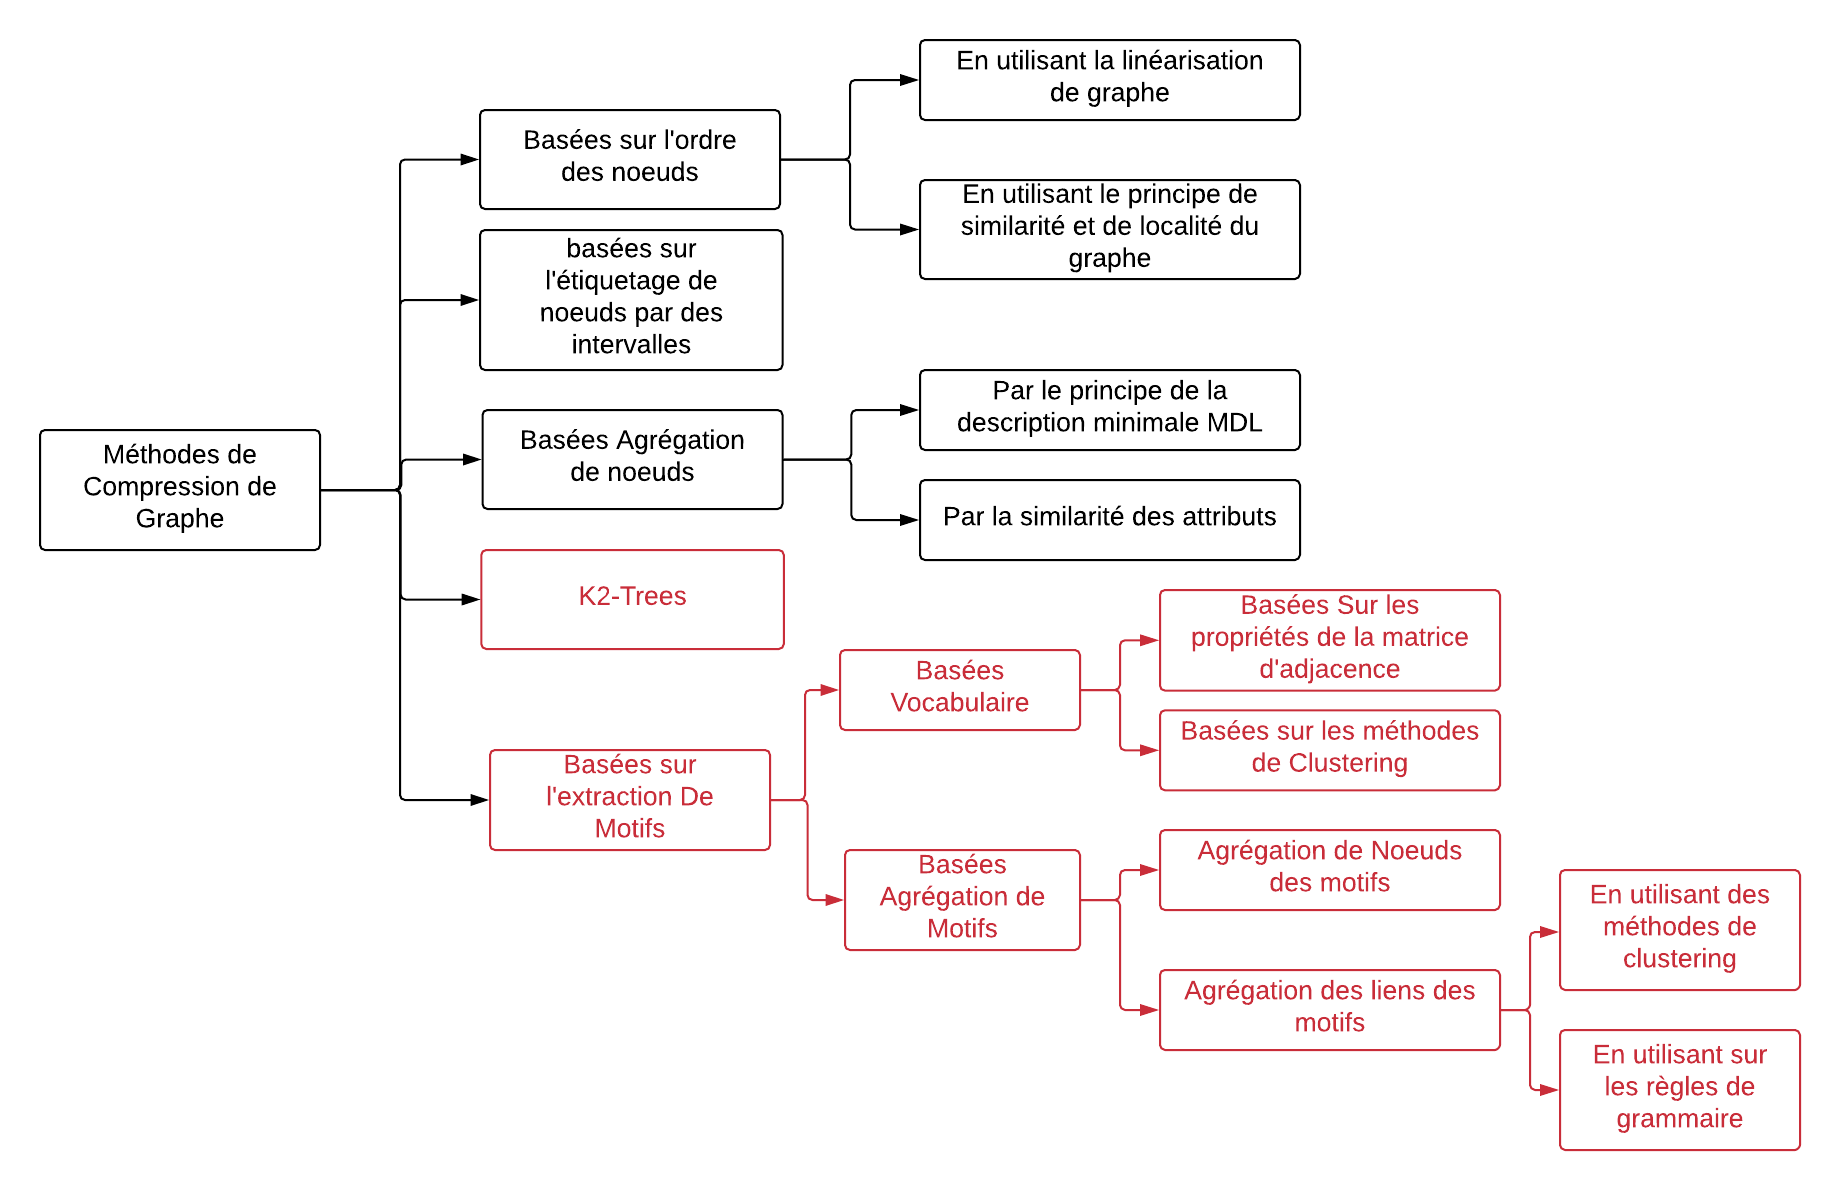
\includegraphics[scale=0.55]{./ressources/image/classif.png}
		\caption{Classification proposées des méthodes de compression}
		\label{classif}
	\end{figure}






			\section{Compression par les K2-Trees}
				$k^2$-tree est une structure de données conçue à l'origine pour la compression des graphes du web. L'algorithme de base a été proposé par Bisaboa et al. dans leur article \textit{$k^2$-trees for Compact Web Graph} \citep{brisaboa2009k}. Elle a été appliquée ensuite dans d'autres types de données tel que les réseaux sociaux \citep{shi2012optimizing}, les données rasters \citep{de2013compact} et les bases de données \gls{rdf} \citep{alvarez2017succinct}.\\

En général, l'algorithme peut être appliqué à n'importe quelle matrice binaire. Dans le cadre de notre étude nous nous intéressons seulement à la matrice d'adjacence d'un graphe.
La compression par les $k^2$-trees exploite les propriétés de la matrice d'adjacence et tire parti des zones vides pour réduire l'espace de stockage et permettre au graphe de tenir en mémoire centrale. Il offre aussi la possibilité de naviguer dans le graphe sans le décompresser, et de répondre aux requêtes de voisinage direct et inverse.

Étant donné une matrice d'adjacence A d'ordre $|n|$, $k^2$-tree la représente sous forme d'un arbre de recherche $k^2$-aires \footnote{Les arbres n-aires sont une généralisation des arbres binaires : chaque nœud a au plus n fils.} de hauteur h = [$log_{k}$ n]. Chaque nœud de l'arbre contient un seul bit avec deux valeurs possibles : 1 pour les nœuds internes et 0 pour les feuilles, sauf le dernier niveau où les feuilles représentent les cases de la matrice A et peuvent prendre une valeur 0 ou 1. Chaque nœud interne de l'arbre a exactement $k^2$ fils.  
Avant la construction de l'arbre, il faut s'assurer que n est une puissance de k. Dans le cas contraire, l'algorithme étend la matrice en rajoutant des zéros à droite et en bas de la matrice. L'ordre de la matrice devient donc $n'= k^{log_{k} n}$.\\

Pour construire l'arbre, $k^2$-tree commence par diviser la matrice en $k^{2}$ sous matrices d'ordre $|n/k|$. La racine correspond à la matrice complète. Chaque sous matrice représente un nœud dans le premier niveau de l'arbre, elle est ajoutée comme un fils à la racine suivant un ordre de gauche à droite et de haut en bas. Le nœud est à 1 si la sous matrice qu'il représente contient au moins un 1, et à 0 si elle ne contient que des 0. Le processus est répété de manière récursive sur les sous matrices représentées par des 1. $k^{2}$ sous matrices sont considérées à chaque subdivision. L'opération est répétée jusqu'à ce que la subdivision atteint les cases de la matrice qui représenterons les feuilles de l'arbre au dernier niveau. 

La figure \ref{k2-trees-exemples} illustre la représentation $k^2$-tree d'une matrice de taille $10 \times 10$, étendue à une  taille $16 \times 16$ pour un k=2 \citep{brisaboa2015efficient}.

\begin{figure}[H]
\begin{center}
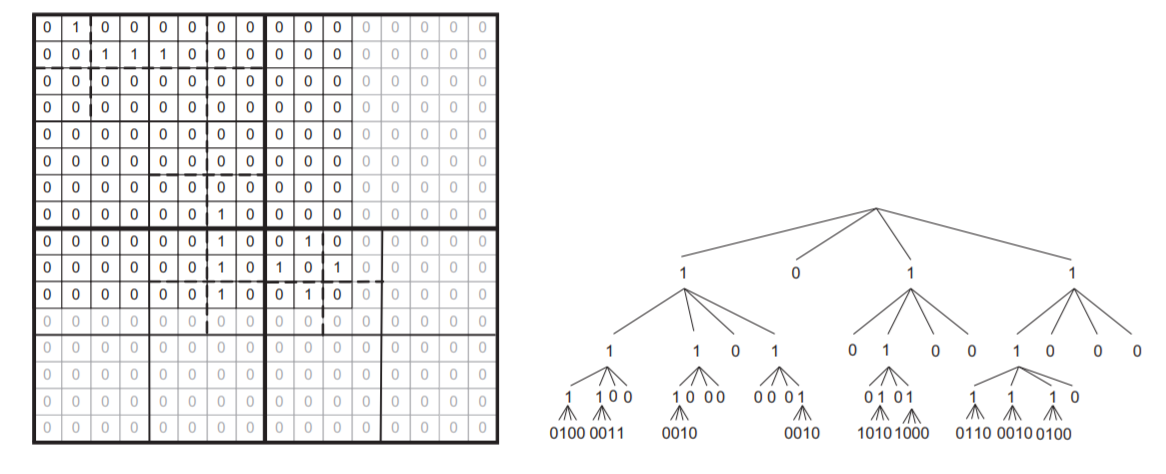
\includegraphics[height=200 pt, width=450 pt]{./ressources/image/k2-trees.png} 
\end{center}
\caption{Exemple de représentation $k^2$-tree}
\label{k2-trees-exemples}
\end{figure}


Pour le stockage de l'arbre, l'algorithme utilise deux tableaux binaires : un tableau T (Tree) contenant tous les nœuds de l'arbre à l'exception du dernier niveau et un tableau L (Leaves) contenant les feuilles du dernier niveau. Les nœuds et les feuilles sont ordonnés selon un parcours en largeur de l'arbre.   
Ci-dessous les deux tableaux T et L de l'exemple précédent (figure \ref{k2-trees-exemples}) : \\
\begin{center}
	T = 1011 1101 0100 1000 1100 1000 0001 0101 1110\\
	L = 0100 0011 0010 0010 1010 1000 0110 0010 0100\\	
\end{center}
Dans le pire des cas, l'espace total pour la description de la structure est $k^2*m(log_{k^2}\frac{n^2}{m}+ \textit{O}(1))$, où n est le nombre de nœuds du graphe et m le nombre de liens. Cependant, pour les graphes réels, l'espace nécessaire pour le stockage est bien meilleur. \\

Dans le même article \citep{brisaboa2009k}, et dans le but d'obtenir un compromis entre la taille de l'arbre et le temps de parcours, les auteurs proposent une hybridation qui consiste à changer la valeur du paramètre k en fonction du niveau de l'arbre en donnant à k une grande valeur au début pour réduire le nombre de niveaux et améliorer ainsi le temps de recherche, et une petite valeur à la fin pour avoir des petites sous matrices et réduire l'espace de stockage.
Pour le stockage de l'arbre, un tableau $T_{i}$ est utilisé pour chaque valeur $k_{i}$, le tableau L reste le même.\\

Plusieurs variantes de l'algorithme de base ont été proposées dans la littérature dont le but était soit d'obtenir un meilleur résultat de compression, soit d'appliquer la méthode sur d'autres types de graphes. Nous allons dans ce qui suit présenter les principaux travaux qui traitent ce sujet.\\

Dans \citep{shi2012optimizing}, les auteurs proposent deux techniques d'optimisation de l'algorithme : la première consiste à trouver un certain ordre des nœuds qui permet de regrouper les 1 de la matrice d'adjacence dans une seule sous matrice au lieu qu'ils soient dispersés de manière aléatoire. La recherche d'un ordre optimal des nœuds n'est pas envisageable. Avec k=2,le problème peut être réduit à un autre problème (min bisection\footnote{Le problème de bissection minimale (MBP) est un problème NP-hard bien connu, qui est destiné à diviser les sommets d'un graphe en deux moitiés égales afin de minimiser le nombre de ces arêtes avec exactement une extrémité dans chaque moitié.}) qui est NP-difficile. Les auteurs utilisent alors un parcourt \newacronym{dfs}{DFS}{Deapth First Search}\gls{dfs}
\footnote{\gls{dfs} : Parcours en profondeurs du graphe}
 avec des heuristiques pour trouver une approximation de l'ordre optimal. Cette optimisation permet de réduire le nombre de nœuds internes de l'arbre et produit ainsi un arbre optimal. La deuxième optimisation est de trouver la valeur de k la plus adéquate pour chaque nœud interne, calculer cette valeur pour chaque nœud peut engendrer un temps de calcul très important. Pour éviter cela, les auteurs affectent la même valeur k pour les nœuds ayant le même parent. 	

Dans un travail ultérieur \citep{brisaboa2014compact}, les auteurs de l'article de base apportent deux améliorations principales de leur méthode dans le but d'optimiser l'espace et le temps de parcours de l'arbre produit. La première est de construire $k^2$ arbres distincts pour les $k_{0}^{2}$ sous matrices du premier niveau. Elle présente plusieurs avantages : (1) l'espace est réduit étant donné que la taille de chaque arbre est en fonction de $\frac{n^2}{k^2}$, (2) le temps de parcours s'améliore puisque T et L sont plus petits. La deuxième amélioration est la compression de L qui consiste à construire un vocabulaire \textit{V} de toutes les sous matrices du dernier niveau sous forme de séquences de bits, les classer par fréquence d'apparition et remplacer leurs occurrences dans L par des pointeurs. Cela permet d'éviter la redondance et de réduire la taille de la structure. Les pointeurs sont représentés par des codes de longueur variable ordonnés, le plus petit correspond à la sous matrice la plus fréquente. Néanmoins, cette représentation ne permet pas un accès direct dans L étant donné qu'une décompression séquentielle est nécessaire pour récupérer une position. Pour remédier à ce problème, les auteurs utilisent le principe de
\newacronym{dac}{DAC}{Directly Addressable Codes}
 \gls{dac}\footnote{\gls{dac} est une technique qui encode une séquence d'entiers ou mots en utilisant une structure à longueur variable, son avantage principale est l'accès direct au mot sans passer par le décodage.} \citep{brisaboa2013dacs} pour garantir un accès rapide au pointeur et conserver ainsi une navigation efficace.\\
Exemple : Pour la figure \ref{k2-trees-exemples}, le vocabulaire et L sont représentés comme suit :\\
\begin{center}
\textit{V}= [0010 0100 0011 1010 1000 0110]\\
L = $c_{1}c_{2}c_{0}c_{0}c_{3}c_{4}c_{5}c_{0}c_{1}$ \\
\end{center}

%\subsubsection{d$k^2$-trees}
Dans \citep{brisaboa2012compressed}, les même auteurs développent la représentation $k^2$-trees pour les graphes dynamiques. Ils proposent une nouvelle structure nommée d$k^2$-trees pour \textit{Dynamique $k^2$-trees} qui offre les même capacités de compression et fonctionnalités de navigation que le cas statique et qui permet également d'avoir des mises à jour sur le graphe. Pour atteindre ces objectifs, d$k^2$-tree remplace la structure statique de $k^2$-tree par une implémentation dynamique. Dans cette nouvelle implémentation, les deux tableaux T et L sont remplacés par deux arbres, nommés $T_{tree}$ et $L_{tree}$ respectivement. Les feuilles de $T_{tree}$ et $L_{tree}$ stockent des parties des bitmaps T et L. La taille de ces feuilles est une valeur paramétrable. Les nœuds internes des deux arbres permettent d'accéder aux feuilles et de les modifier.
Chaque nœud interne de $T_{tree}$ contient trois(03) éléments : deux compteurs b et o, qui contiennent respectivement le nombre de bits et le nombre de "1" stockés dans les feuilles descendantes de ce nœud, et un pointeur P vers le nœud fils. Les nœuds internes de $L_{trees}$ sont similaires sauf qu'ils ne contiennent que b et P. Avec cette structuration, $T_{tree}$ et $L_{tree}$ permettent la mise à jour directe de l'arbre $k_2-tree$ dans le cas l'ajout et la suppression des liens dans le graphe.\\
La figure \ref{dk2-trees} présente une représentation d$k^2$-tree \citep{brisaboa2012compressed}: 
\begin{figure}[H]
\begin{center}
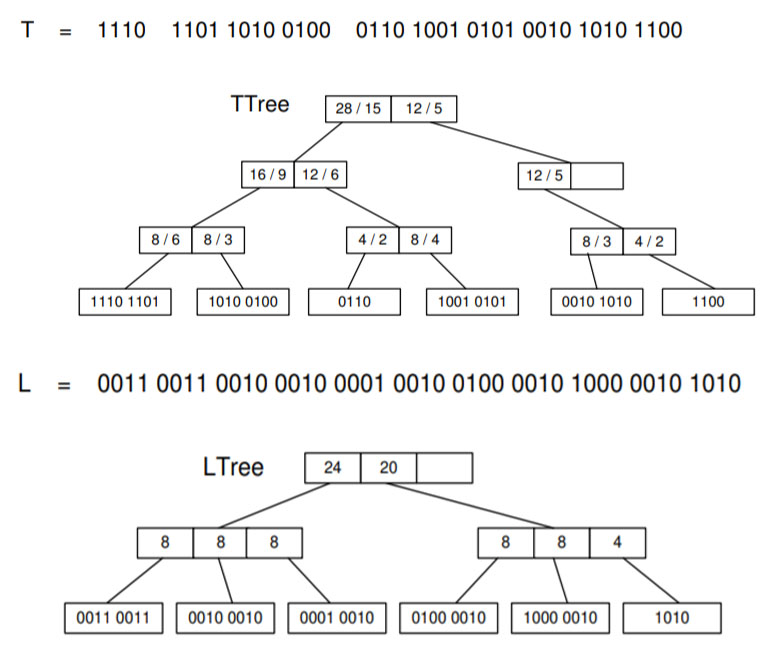
\includegraphics[scale=0.7]{./ressources/image/dk2-trees.jpg} 
\end{center}
\caption{Exemple d'une représentation d$k^2$-tree}
\label{dk2-trees}
\end{figure}

%\subsubsection{$k^n$-trees}
 Sandra et al. \citep{de2013compact} présentent $k^n$-tree, une généralisation des $k^2$-tree pour les problèmes multidimensionnels. Cette méthode possède plusieurs applications. Elle est utilisée pour représenter les bases de données multidimensionnelles, les données rasters et les graphes dynamiques. $k^n$-tree repose sur $k^2$-tree pour représenter une matrice à n-dimensions (dites \textit{tensor} en Anglais). La matrice est décomposé en $k^n$ sous-matrices de même taille, comme suit : sur chaque dimension, K-1 hyperplans devisent la matrice dans les positions i*$\frac{n}{K}$,pour $i \in [1, K-1]$. Une fois les dimensions partitionnées, $k^n$ sous-matrices sont induites, elles sont représentées par des nœuds dans l'arbre comme dans l'algorithme de base. Les structures utilisées pour le stockage sont aussi les mêmes (T et L).
En posant n=3, la méthode peut être appliquée sur les graphes dynamiques ou temporels. Ce type de graphe est représenté par une grille à 3 dimensions $X \times Y \times T$, où les deux premières dimensions représentent les nœuds de départ et de destination, et la troisième dimension représente le temps. 
La figure \ref{kn-trees} présente une représentation $k^3$-tree d'un graphe dynamique \citep{de2014new}.

\begin{figure}[H]
\begin{center}
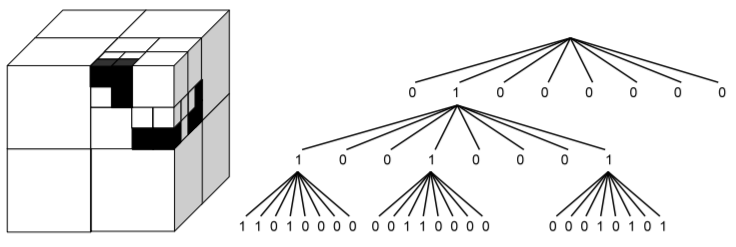
\includegraphics[height=100 pt, width=380 pt]{./ressources/image/kn-trees.png} 
\end{center}
\caption{Exemple d'une représentation $k^3$-tree}
\label{kn-trees}
\end{figure}



%\subsubsection{$K^2$-tress1 }
La représentation de base des arbres k2-trees regroupe seulement les zones de zéros, puisqu'elle a été conçue au début pour les graphes du web qui possèdent une matrice d'adjacence extrêmement creuse. Dans \citep{de2014new}, Les auteurs proposent d'étendre cette représentation en regroupant les zones de "1" également. L'idée générale est d'arrêter la décomposition de la matrice d'adjacence quand une zone unie est trouvée, à savoir des zéros ou des uns. Pour distinguer entre les différents nœuds, une représentation quadtree est utilisée \citep{de1997computational}. Une couleur est attribuée à chaque nœud, blanc pour une zone de zéro, noir pour une zone de uns et gris pour les nœuds internes, i.e, les zones contenant des uns et des zéros. Pour le stockage des nœuds, les auteurs proposent quatre encodages présentés dans ce qui suit : 

\begin{enumerate}[label=$\bullet$]
\item \textbf{ $k^2$-$trees1^{2-bits-naive}$ :} Dans cet encodage, deux bits sont utilisés pour représenter chaque type de nœud. L'attribution des bits n'est pas arbitraire, le premier bit du poids fort indique si le nœud est un nœud interne (0) ou une feuille (1), le deuxième détermine si les feuilles sont blanches (0) ou noires (1). Nous aurons donc : "10" pour les nœuds gris, "01" pour les nœuds noirs et "00" pour les nœuds blancs. Notant que les feuilles du dernier niveau sont représentées par un seul bit.
Après le codage, le premier bit de chaque nœud sauf ceux du dernier niveau est stocké dans T, un autre tableau $T'$ est créé pour sauvegarder le deuxième bit. Les nœuds du dernier niveau sont stockés dans L.
\item \textbf{ $k^2$-$tree1^{2-bits}$ :} Le même principe que l'encodage précédant sauf que les nœuds gris sont représentés par un seul bit, toujours à "1". Le tableau $T'$ va contenir dans ce cas la couleur des feuilles ce qui va réduire la taille de la structure.

\item \textbf{ $k^2$-$tree1^{DF}$ :} Cet encodage est similaire à $k^2$-$trees1^{2-bits}$, mais il utilise un seul bit pour les nœuds blancs et deux bits pour les nœuds noirs et gris, compte tenue de la fréquence des nœuds blancs dans les graphes du monde réel par rapport aux autres. Nous aurons donc : "0" pour les nœuds blancs, "10" pour les nœuds gris et "11" pour les nœuds noirs.

\item \textbf{ $k^2$-$tree1^{5-bits}$ :} Le dernier encodage repose sur la représentation de base. Un nœud blanc est représenté par "0", un nœud noir ou gris par "1", exactement comme le $k^2$-tree d'origine. Pour identifier un nœud noir (zone de uns), il sera représenté par une combinaison impossible : $k^2$ fils de "0" sont ajoutés aux nœuds noirs pour les distinguer.
\end{enumerate}


La figure \ref{k2-trees1-exemple} illustre une représentation $k^2$-tress1 avec les quatre encodages \citep{de2014new} : 


\begin{figure}[H]
\begin{center}
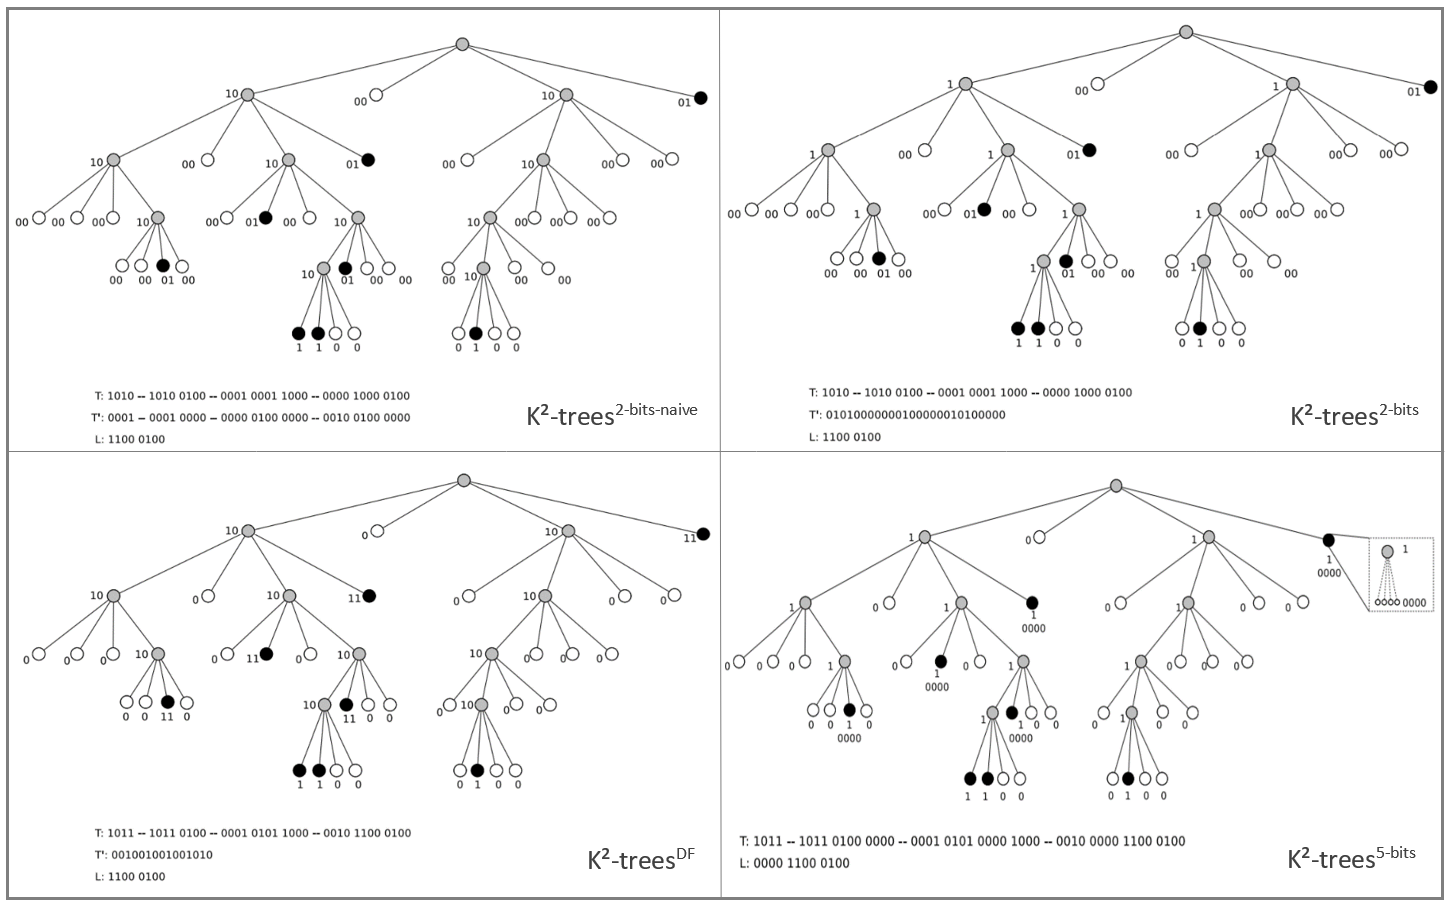
\includegraphics[height=300 pt, width=450 pt]{./ressources/image/k2-trees1.png} 
\end{center}
\caption{Exemple d'une représentation $k^2$-tree1 avec les quatre encodages}
\label{k2-trees1-exemple}
\end{figure}


%\subsubsection{Delta-$K^2$-tress }

Dans \citep{zhang2014delta}, les auteurs proposent Delta-$k^2$-tree, une variante qui exploite la propriété de similarité entre les nœuds voisins du graphe pour réduire le nombre de uns dans la matrice d'adjacence. Notons par \textit{Matrix} la matrice d'adjacence, Delta-$k^2$-trees construit une nouvelle matrice appelée \textit{Delta-matrix}, une ligne \textit{i} de \textit{Delta-matrix} va contenir la différence entre les deux lignes \textit{Matrix}[i] et  \textit{Matrix}[i-1] si cela décroit le nombre de uns sinon elle sera égale à \textit{Matrix}[i], comme suit: \\

$\left\{
\begin{array}{llcl}
\textbf{Si}\ \ count1s(matrix[i]) < countDif(matrice[i],matrix[i-1])\\
\ \ \ \ Delta-matrix[i]  := matrix[i]  \\
\textbf{Sinon} & & &\\
\ \ \ \ Delta-matrix[i]  := matrix[i] \bigoplus matrix[i-1] & 
\end{array}
\right.$\\

Où \textit{count1s} compte le nombre de 1 dans une ligne, \textit{countDif} compte le nombre de bits différents entre deux lignes et $\bigoplus$ représente le "ou exclusif".

Pour déterminer si une ligne est identique à celle de la matrice d'adjacence ou non, un tableau D est utilisé : Si D[i]=1 la ligne est identique, sinon c'est une ligne de différence.\\
La matrice \textit{Delta-matrix} contient moins de uns que la matrice d'adjacence, d'où elle est plus creuse, ce qui permet de réduire la taille de la structure et avoir un meilleur taux de compression. Cependant le temps de parcours est plus grand car pour accéder à certaines lignes (lignes de différence), le graphe doit être décompressé et la matrice d'adjacence reconstituée.\\
La figure \ref{k2-trees-delta} présente un exemple de la représentation Delta-$k^2$-tree \citep{zhang2014delta}.


\begin{figure}[H]
\begin{center}
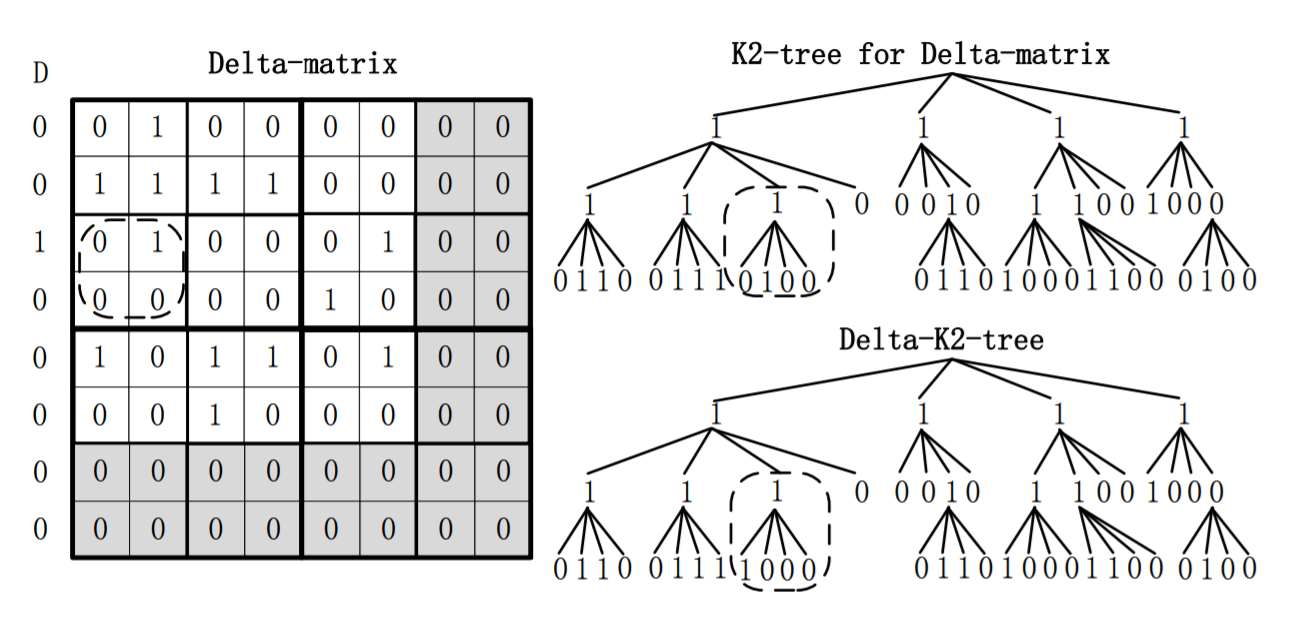
\includegraphics[height=150 pt, width=380 pt]{./ressources/image/k2-trees-delta.png} 
\end{center}
\caption{Exemple d'une représentation Delta-$k^2$-tree}
\label{k2-trees-delta}
\end{figure}

%\subsubsection{$K^2$-treaps }
$K^2$-treap est une autre variante de $k^2$-tree, elle a été proposée dans \citep{brisaboa2014k}. Cette variante combine les $k^2$-trees avec une autre structure de données appelée treap \footnote{Les Treaps sont des arbres de recherche binaire avec des nœuds ayant deux attributs : clé et priorité. La recherche dans ces arbres s'effectue selon ces attributs.} \citep{aragon1989randomized}. Les auteurs appliquent cette méthode sur des grilles multidimensionnelles comme 
\newacronym{olap}{OLAP}{Online Analytical Processing}
\gls{olap} pour pouvoir les stocker et répondre efficacement aux requêtes top-K \citep{badr2013traitement}. La méthode peut être également appliquée sur les graphes pondérés, où chaque case de la matrice d'adjacence du graphe comporte le poids de l'arête qu'elle représente au lieu d'un 1.
Comme dans l'algorithme de base, une décomposition récursive en $k^2$ sous-matrices est appliquée sur la matrice d'adjacence et un arbre $k^2$-air est construit comme suit : la racine de l'arbre va contenir les coordonnées ainsi que la valeur de la cellule ayant le plus grand poids de la matrice. La cellule ajoutée à l'arbre est ensuite supprimée de la matrice. Si plusieurs cellules ont la même valeur maximale, l'une d'elles est choisie au hasard. Ce processus est répété récursivement sur chaque sous matrice. La procédure continue sur chaque branche de l'arbre jusqu'à ce qu'on tombe sur les cellules de la matrice d'origine ou sur une sous matrice complètement vide (contient que des zéros).\\
La figure \ref{k2-treaps} suivante illustre la représentation $k^2$-treap d'un graphe pondéré \citep{badr2013traitement} :

\begin{figure}[H]
\begin{center}
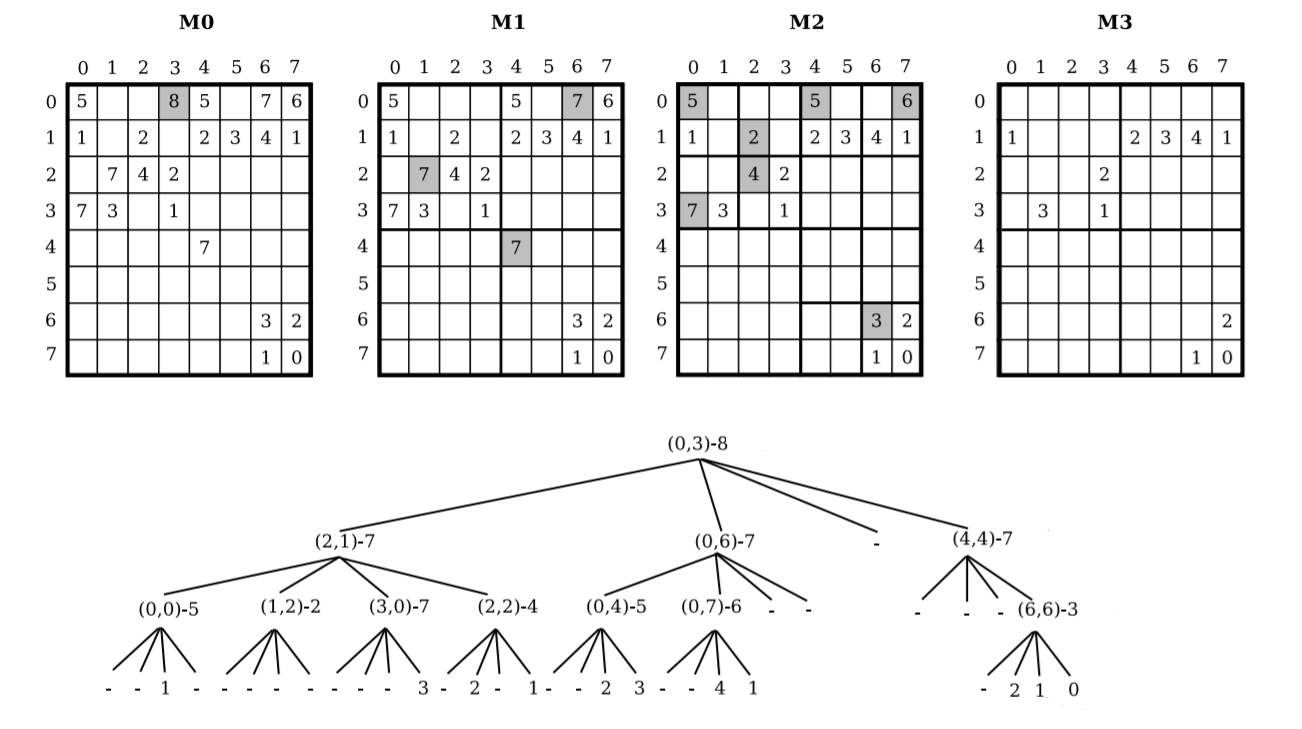
\includegraphics[height=200 pt, width=380 pt]{./ressources/image/k2-treaps.png} 
\end{center}
\caption{Exemple d'une représentation $k^2$-treap d'un graphe pondéré}
\label{k2-treaps}
\end{figure}

Pour avoir une bonne compression, $k^2$-treap effectue des transformations sur les données stockées. La première transformation consiste à changer les coordonnées représentées dans l'arbre en des coordonnées relatives par rapport à la sous matrice actuelle. La deuxième est de remplacer chaque poids dans l'arbre par la différence entre sa valeur et celle de son parent.\\
Trois structures de données sont utilisées pour sauvegarder les coordonnées et les valeurs des cellules ainsi que la topologie de l'arbre. Chaque structure est détaillée dans ce qui suit :
\begin{itemize}
\item \textit{Listes de coordonnées locales :} La séquence de coordonnées de chaque niveau \textit{l} de l'arbre est stockée dans une liste \textit{coord}[\textit{l}].
\item \textit{Liste des valeurs : } Le parcours de l'arbre se fait en largeur, la séquence des valeurs récupérées est stockée dans une liste nommée \textit{values}. Un tableau nommé \textit{first} est utilisé pour sauvegarder la position début de chaque niveau dans \textit{values}.
\item \textit{L'arbre :} La structure de l'arbre $k^2$-treap est sauvegardée avec un arbre $k^2$-tree, les nœuds contenant des valeurs dans $k^2$-treap sont représentés par des uns et les nœuds vides par des zéros. Pour le stockage de l'arbre, un seul tableau T est utilisé. 
\end{itemize}

La figure \ref{k2-treaps-structure} représente les structures de données utilisées pour le stockage de l'arbre de la figure \ref{k2-treaps} précédente \citep{badr2013traitement} :

\begin{figure}[H]
\begin{center}
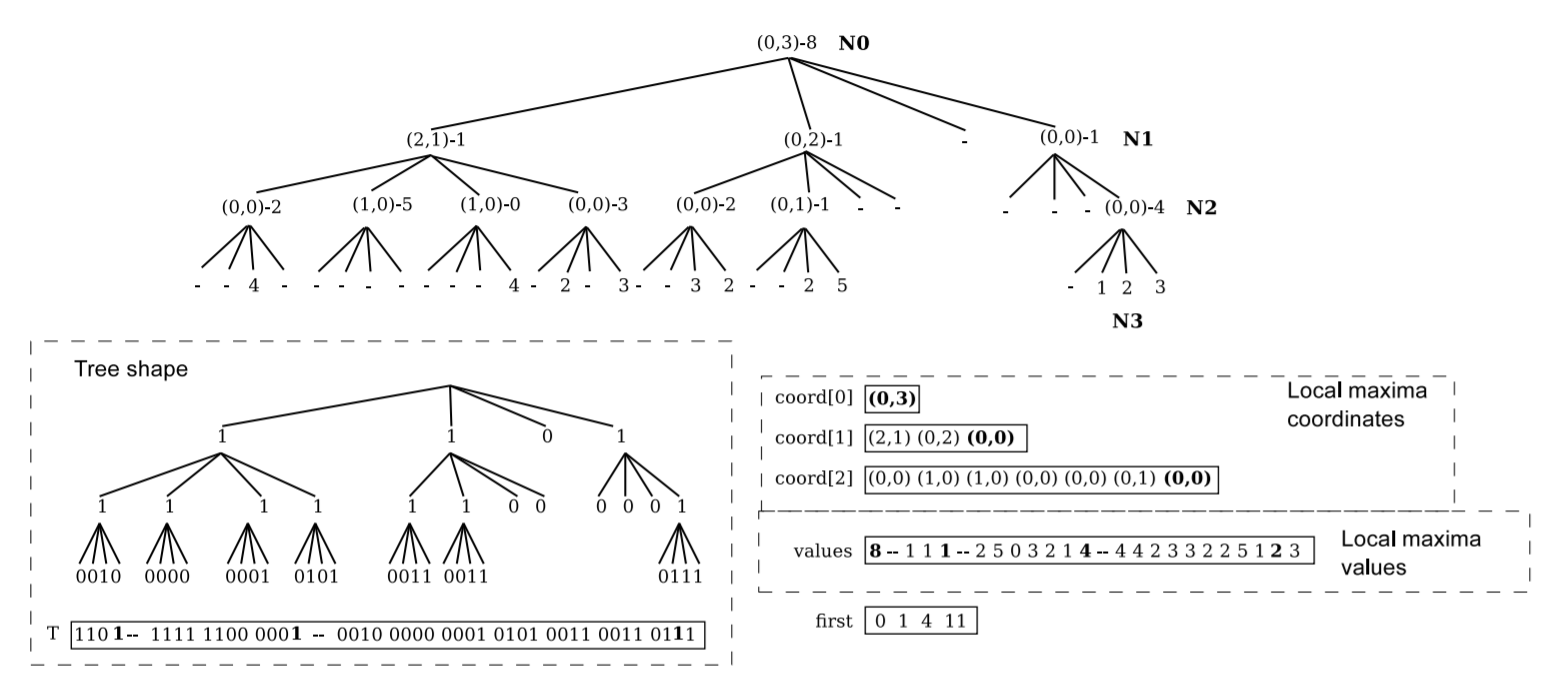
\includegraphics[height=200 pt, width=380 pt]{./ressources/image/k2-treaps-structure.png} 
\end{center}
\caption{Structures de données pour une représentation $k^2$-treap}
\label{k2-treaps-structure}
\end{figure}

%\subsubsection{I$k^2$-trees}
Garcia et al. \citep{garcia2014interleaved} proposent I$k^2$-tree pour Interleaved $k^2$-tree. Elle est appliquée sur les bases de données RDF ainsi que sur les graphes dynamiques. Dans les graphes dynamiques, les deux premières dimensions correspondent aux nœuds source et destination et la troisième dimension reflète le temps. Le graphe est donc défini par |T| matrices d'adjacence prisent à des instants $t_k$ différents. I$k^2$-tree représente les matrices simultanément. Chaque matrice est représentée par un arbre $k^2$-tree et ils sont par la suite regroupés dans un seul arbre. Chaque nœud de l'arbre obtenu représente une sous-matrice comme dans l'algorithme de base, sauf qu'au lieu d'utiliser un seul bit, I$k^2$-tree utilise 1 à |T| bits pour représenter le nœud. Le nœud racine contient |T| bits. Le nombre de bits de chaque fils dépend du nombre de uns de son parent. L'arbre finale est toujours stocké avec deux tableaux : T et L.
La figure \ref{Ik2-trees} est un exemple de I$k^2$-tree appliqué sur un graphe dynamique représenté dans trois instants \citep{garcia2014interleaved} :

\begin{figure}[H]
\begin{center}
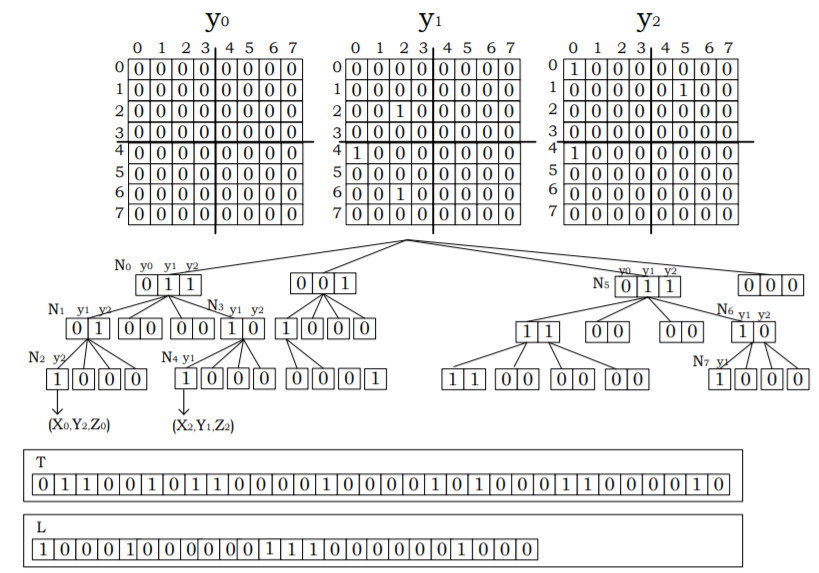
\includegraphics[scale=0.55]{./ressources/image/Ik2-trees.png} 
\end{center}
\caption{Exemple d'une représentation I$k^2$-tree}
\label{Ik2-trees}
\end{figure}

%\subsubsection{diff I$k^2$-trees}
Une variante de I$k^2$-tree appelée Differential I$k^2$-tree a été étudiée dans \citep{alvarez2017succinct}. Elle vise à améliorer le taux de compression en représentant uniquement les changements survenus sur le graphe à un instant $t_i$ au lieu d'une instance complète : à l'instant $t_0$, une capture complète du graphe (matrice d'adjacence) est stockée. À l 'instant $t_k$, pour k>0, seules les arrêtes qui changent de valeurs entre $t_{k-1}$ et $t_k$ sont stockées. Les matrices sont représentées à la fin de la même manière que I$k^2$-tree. La limite de cette représentation est que la structure doit être décompressée lors d'une requête.
La figure \ref{Ik2-trees-diff} montre un exemple d'une représentation diffI$k^2$-trees \citep{alvarez2017succinct}.

\begin{figure}[H]
\begin{center}
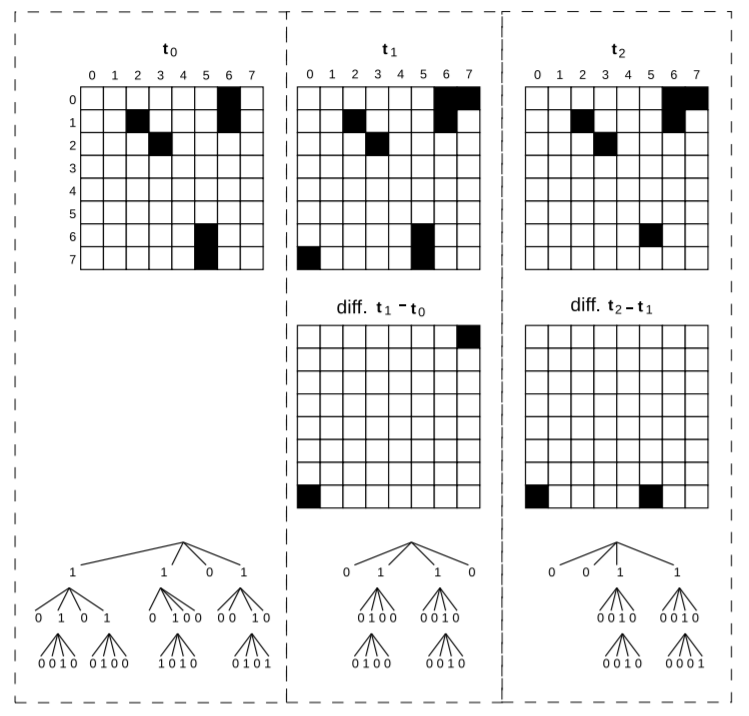
\includegraphics[scale=0.8]{./ressources/image/Ik2-trees-diff.png} 
\end{center}
\caption{Exemple d'une représentation diff I$k^2$-tree}
\label{Ik2-trees-diff}
\end{figure}

%\subsubsection{Att $K^2$-trees }
Dans \citep{alvarez2018compact}, les auteurs étendent la représentation $k^2$-tree pour les bases de données orientées graphes. Ces graphes sont étiquetés, attribués, orientés et ont des arêtes multiples. Ils présentent le graphe sous forme d'une nouvelle structure intitulée Att$k^2$-tree pour Attributed $k^2$-trees.
La figure \ref{k2-trees-att-graphe} montre un exemple de graphe pris en compte par Att$K^2$-tree \citep{alvarez2018compact}.

\begin{figure}[H]
\begin{center}
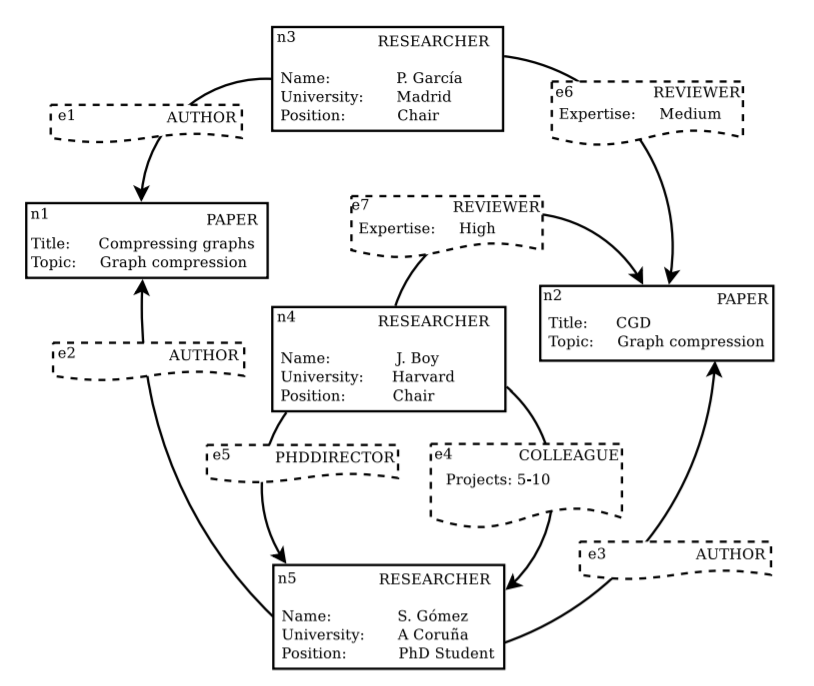
\includegraphics[height=200 pt, width=280 pt]{./ressources/image/k2-trees-att-graphe.png} 
\end{center}
\caption{Exemple d'un graphe étiqueté, attribué, orienté et multiple}
\label{k2-trees-att-graphe}
\end{figure}

\textbf{Structures de données :} La représentation obtenue par la compression est composée d'un ensemble d'arbres $k^2$-tree et d'autres structures supplémentaires. Le graphe est représenté par trois composantes: un schéma de données, les données incluses dans les nœuds et les liens et finalement la relation entre les éléments du graphe. Chaque composant est présenté dans ce qui suit :
\begin{itemize}
\item \textit{Schéma : } Ce composant gère les étiquettes et les attributs de chaque type d'éléments, il joue le rôle d'un index dans la représentation. Il est composé de :
\begin{description}
\item[Un schéma de nœuds :] représenté par un tableau qui contient les étiquettes des nœuds ordonnées lexicographiquement. Un identifiant est attribué à chaque nœud du graphe selon l'ordre du tableau, les \textit{$m_1$} nœuds possédant la première étiquette du tableau vont avoir des identifiants de 1 à \textit{$m_1$}, les \textit{$m_2$} nœuds avec la deuxième étiquette du tableau vont avoir des identifiants de \textit{$m_1$}+1 à \textit{$m_1$}+\textit{$m_2$} et ainsi de suite. Chaque entrée du tableau va ainsi stocker le plus grand identifiant portant son étiquette, cela permet de trouver l'étiquette d'un nœud à travers son identifiant.
\item[Un schéma d'arêtes :] Comme dans le cas des nœuds, un tableau est utilisé pour stocker les étiquettes des arêtes avec le même principe.  
\end{description}
Le schéma est le point de départ de la représentation, il permet d'obtenir l'étiquette d'un nœud ou d'une arête, et d'accéder à ses attributs.
\item \textit{Données :} Ce composant contient toutes les valeurs que peut prendre un attribut dans le graphe. Un attribut peut être représenté de deux façons différentes selon sa fréquence d'apparition, on distingue donc deux types d'attributs :
\begin{description}
\item[Attributs rares :] Ce sont les attributs qui prennent généralement des valeurs différentes à chaque apparition, ils sont stockés dans des listes et indexés avec l'identifiant de l'élément.
\item[Attributs fréquents :] Ce type d'attributs est sauvegardé dans deux matrices, une pour les attributs des nœuds et l'autre pour les attributs des liens. Les matrices sont stockées sous forme d'arbres $k^2$-trees.
\end{description}
La figure \ref{k2-trees-att-schema} illustre les deux composants schéma et données de la représentation Att$k^2$-trees  de la figure \ref{k2-trees-att-graphe} \citep{alvarez2018compact}:
\begin{figure}[H]
\begin{center}
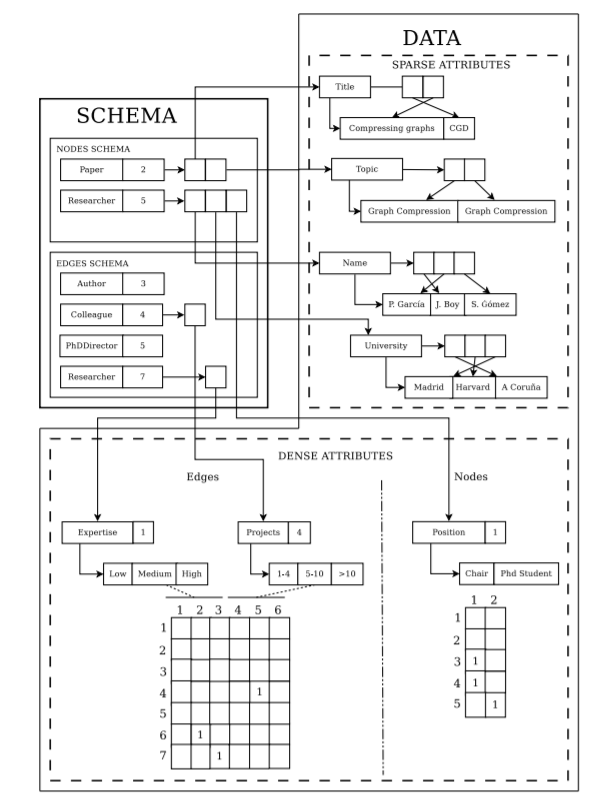
\includegraphics[scale=0.7]{./ressources/image/k2-trees-att-schema.png} 
\end{center}
\caption{Exemple d'une représentation Att$k^2$-tree (1/2)}
\label{k2-trees-att-schema}
\end{figure}


\item \textit{Relations :} C'est le dernier composant de Att$k^2$-tree, il stocke les relations entre les nœuds et les arêtes du graphe en utilisant un arbre $k^2$-tree et d'autres structures pour sauvegarder les identifiants des arêtes ainsi que les arêtes multiples. Les structures supplémentaires sont les suivantes :
\begin{description}
\item[Multi :] Un tableau qui indique si l'arête est multiple ou non.
\item[Firt :] Un tableau qui donne l'identifiant de l'arête, ou de celui de la première dans le cas d'une arrête multiple.
\item[Next :] Un tableau qui contient les identifiants des arêtes multiples restantes.
\end{description}
La figure \ref{k2-trees-att-relation} donne la représentation Att$k^2$-tree des relations du graphe de la figure \ref{k2-trees-att-graphe} \citep{alvarez2018compact}:
\begin{figure}[H]
\begin{center}
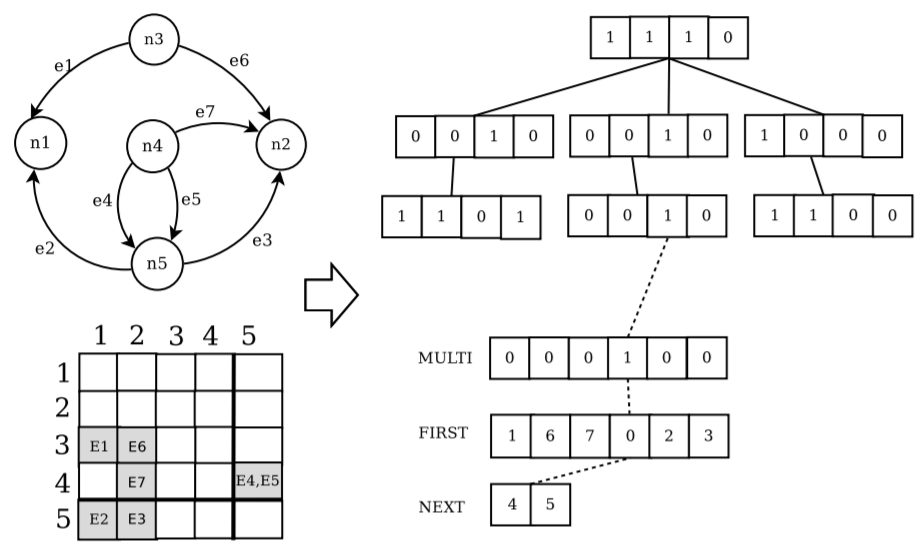
\includegraphics[height=200 pt, width=280 pt]{./ressources/image/k2-trees-att-relation.png} 
\end{center}
\caption{Exemple d'une la représentation Att$k^2$-tree (2/2)}
\label{k2-trees-att-relation}
\end{figure} 
\end{itemize}

%\subsubsection{dynAtt$k^2$-trees }
Dans le même article \citep{alvarez2018compact}, les auteurs étendent Att$k^2$-tree pour les graphes dynamiques. Ils proposent une nouvelle variante appelée dynAtt$k^2$-tree qui supporte le changement dans les attributs et les liens du graphe. Comme Att$k^2$-tree, dynAtt$k^2$-tree représente le graphe avec trois composantes : Schémas, données et relations. Les composantes sont semblables à ceux de Att$k^2$-tree mais avec certaines amélioration vue la nature dynamique du graphe.\\
\textbf{Structure de données : } 
\begin{itemize}
\item \textit{Schéma :}  En ce qui concerne les nœuds, leurs étiquettes sont stockées dans une liste dynamique ordonnée lexicographiquement. En outre, une séquence dynamique est utilisée pour sauvegarder le type de chaque nœud. Elle est stockée ensuite sous forme d'un arbre d'ondelettes \footnote{Ou wavelet en anglais, est un arbre binaire équilibré qui contient des données compressées dans une représentation optimale.} \citep{grossi2003high}. Le même principe est appliqué sur les arrêtes. 
\item \textit{Données :} Les attributs rares sont stockés dans des listes dynamiques, quant aux attributs fréquents, ils sont sauvegardés avec des arbres d$k^2$-trees (un arbre pour chaque attribut).
\item \textit{Relations :} Le stockage des relations se fait à l'aide d'un d$k^2$-tree et des tableaux dynamiques pour stocker les identifiants des arêtes et les arêtes multiples.
\end{itemize}





























				\textbf{Synthèse des méthodes de compression basée sur les $K^2$-trees }

Nous avons présenter dans les parties précédentes les différentes méthodes de compressions basées sur la représentation $k^2$-trees existantes, et expliquer le principes de fonctionnement de chaqu'une d'elles. Nous allons par la suit comparer entre ces méthodes et résumer nos recherche.
Une présentation synthétique de notre étude est fournie dans le tableau \ref{K2-trees-table}. Chaque ligne du tableau représente une méthode, tandis que chaque colonne
représente un aspect susceptible d’être utilisé dans la méthode (type de graphe, type de compression, structure en sortie). Nous constatons que toutes les méthodes de cette classe sont des méthodes de compression sans perte qui supportent les graphes orientés et non orientés, cependant nous remarquons une variation dans l'aspect temporelle, certains méthodes sont destinées aux graphes statiques comme $k^2$-trees de base et $k^2$-trees1, tandis que d'autres sont appliquées aux graphes dynamiques comme $k^n$-trees et d$k^2$-trees. Certains méthodes se distinguent aussi par le type de graphe comme $k^2$-treaps qui s'applique aux graphes pondérés et Att$k^2$-trees qui accepte les graphes étiquetés, attribués et multiples. Nous observons aussi que toutes les méthodes donnent en sortie une représentation succincte. le tableau résume aussi les résultats de l'application des méthodes sur des graphe de tests. Les figures \ref{eu2005-k2} et \ref{k2-taux} sont des représentations visuelles des ces résultats.\\

La figure \ref{eu2005-k2} représente les résultats obtenues par l'application des méthodes de compressions basées sur les $k^2$-trees sur le graphe eu-2005 en tenant compte de l’ordre chronologique de leurs apparitions. Les résultats sont sous forme de nombre de bits par liens. Nous remarquons que la première méthode de base donne un résultat de compression de 5.2bpl, ce nombre a diminuer avec l'apparition des améliorations et des nouvelles méthodes. Nous constatons alors une amélioration contenue de l'efficacité de ces méthodes de manière générale surtout avec les amélioration proposées par \citep{brisaboa2014compact} et Delta$k^2$-trees où le nombre de bits atteint approximativement 3.22 bits par liens.

 \begin{figure}[H]
		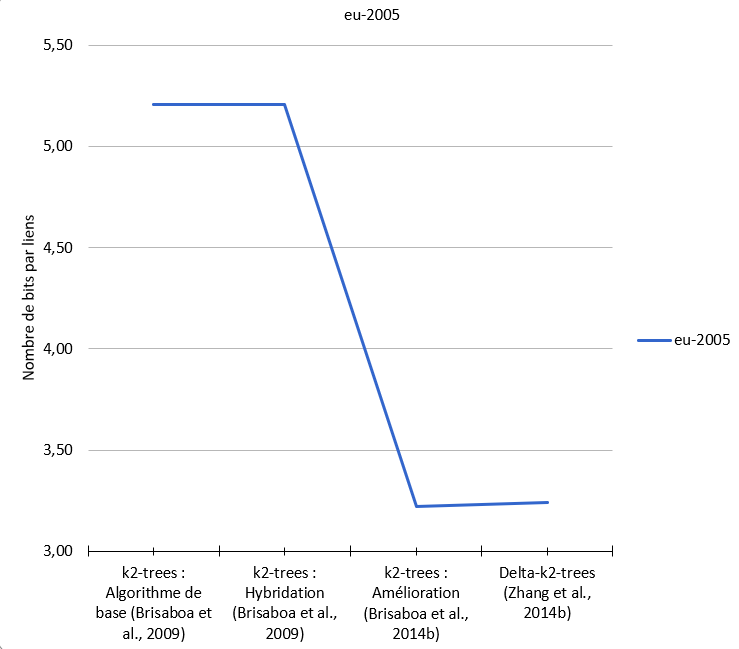
\includegraphics[height=10.5cm, width=16cm]{./ressources/image/eu2005-k2.png}
		\caption{Comparaison des performances des méthodes basées sur les $k^2$-trees appliquées sur le graphe eu2005 selon le nombre de bits par liens}
		\label{eu2005-k2}
	\end{figure}
	
A partir de la \ref{K2-trees-table} qui présente les résultats de l'application de différentes méthodes sur quatre graphes de test (CommNet, cond-mat, eu-2005, movilens10M) en fonction du taux de compression. Nous remarquons que entre $k^2$-trees et $k^2$-trees1, la méthode $k^2$-trees est nettement meilleure, cela s'explique par le fait que les graphes du web sont représentés par des matrices creuses et $k^2$-trees1 est mieux adaptée au matrices avec des zones de uns comme les matrices d'images par exemples.	Pour les graphes dynamique, nous observons que $k^n$-trees donne de bons résultats par rapport à I$k^2$-trees mais avec une légère différence. Pour les graphes attribués, Att$k^2$-trees donne un très bon résultat avec un taux de compression de 93\%. 
	\begin{figure}[H]
		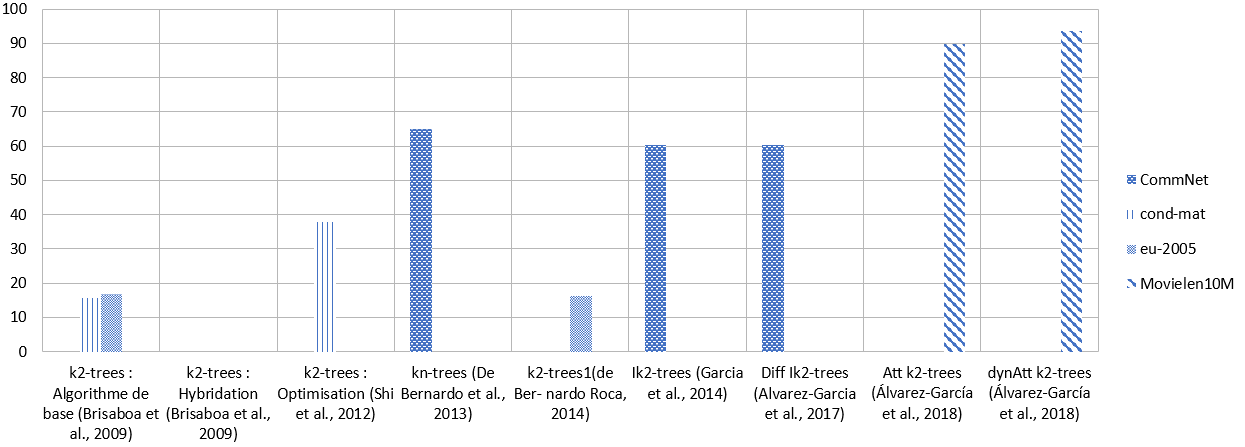
\includegraphics[height=9cm, width=18cm]{./ressources/image/k2-taux.png}
		\caption{comparaison entre les méthodes basées sur les $k^2$-trees en fonction du taux de compression}
		\label{k2-taux}
	\end{figure}
	


    
 												
														\begin{landscape}
								\begin{table}
									\begin{tabular}{|C{3cm}|c|c|c|c|c|c|c|c|c|c|c|c|c|}
										\hline
										\multirow{2}{*}[-25pt]{     Article   }  & \multicolumn{5}{c|}{Graphe en entrée} & \multicolumn{2}{c|}{Compression} & \multicolumn{2}{c|}{Structure en sortie} & \multirow{2}{*}[-25pt]{Graphe de test} & \multirow{2}{*}[-25pt]{Résultat }  \\ \cline{2-10}
				     & \rotatebox[origin=c]{90}{ Orienté }  & \rotatebox[origin=c]{90}{ Non orienté } & \rotatebox[origin=c]{90}{ Statique } & \rotatebox[origin=c]{90}{ Dynamique } & \rotatebox[origin=c]{90}{ Autre Propriétés } &  \rotatebox[origin=c]{90}{ Avec perte } & \rotatebox[origin=c]{90}{ Sans perte } & \rotatebox[origin=c]{90}{ Succincte } & \rotatebox[origin=c]{90}{ Structurelle } & & \\ \hline				%%%%%%Fin du header
				
\hline  $k^2$-trees : Algorithme de base
   \citep{brisaboa2009k} 
   & \cmark & \cmark & \cmark & \xmark &  & \xmark &  \cmark & \cmark & \xmark	 & 		
	\begin{minipage}[t]{0.15\textwidth}
	eu-2005\\
	
	cond-mat
  \end{minipage}	
										 &
	\begin{minipage}[t]{0.4\textwidth}
	 5.21 bits/lien \\
	 taux de compression : 16.88\% \\
	 taux de compression : 15.58\% 
  \end{minipage}	\\

\hline $k^2$-trees : Hybridation \citep{brisaboa2009k} & \cmark & \cmark & \cmark & \xmark &  & \xmark &  \cmark & \cmark & \xmark  & 
										\begin{minipage}[t]{0.15\textwidth}
	eu-2005
  \end{minipage}	
										 &
	\begin{minipage}[t]{0.4\textwidth}
	 5.21 bits/lien 
  \end{minipage}	\\  
\hline $k^2$-trees : Optimisation \citep{shi2012optimizing} & \cmark & \cmark & \cmark & \xmark &  & \xmark &  \cmark & \cmark & \xmark  & 
\begin{minipage}[t]{0.15\textwidth}
	cond-mat
  \end{minipage}	
										 &
	\begin{minipage}[t]{0.4\textwidth}
	
	 taux de compression : 37.96\% 
  \end{minipage}	\\
  			\hline
  			
\hline $k^2$-trees : Amélioration \citep{brisaboa2014compact} & \cmark & \cmark & \cmark & \xmark &  & \xmark &  \cmark & \cmark & \xmark  & 
  				\begin{minipage}[t]{0.15\textwidth}
	eu-2005
  \end{minipage}	
										 &
	\begin{minipage}[t]{0.4\textwidth}
	
	 3.22 bits/lien
  \end{minipage}	\\
  				
  				\hline  		
  			
\hline d$k^2$-trees \citep{brisaboa2012compressed} & \cmark & \cmark & \xmark & \cmark &  & \xmark &  \cmark & \cmark & \xmark  &
  				\begin{minipage}[t]{0.15\textwidth}
	eu-2005
  \end{minipage}	
										 &
	\begin{minipage}[t]{0.4\textwidth}
	
	 6.2 bits/lien
  \end{minipage}	\\
  \hline 
  			
\hline $k^n$-trees \citep{de2013compact} & \cmark & \cmark & \xmark & \cmark & & \xmark & \cmark & \cmark & \xmark  &
  				\begin{minipage}[t]{0.15\textwidth}
	CommNet
  \end{minipage}	
										 &
	\begin{minipage}[t]{0.4\textwidth}
	
	 taux de compression : 65.16\% 
  \end{minipage}	\\
  \hline  	

  			

  					
 	
  			
									\end{tabular}
									\caption{Synthèse des méthodes de compression par $k^2$-trees.}									
									
								\end{table}
								
							\end{landscape}
							
							
							
%% deuxiéme tableau

					\begin{landscape}
								\begin{table}
									\begin{tabular}{|C{3cm}|c|c|c|c|c|c|c|c|c|c|c|c|c|}
										\hline
										\multirow{2}{*}[-25pt]{Article}  & \multicolumn{5}{c|}{Graphe en entrée} & \multicolumn{2}{c|}{Compression} & \multicolumn{2}{c|}{Structure en sortie} & \multirow{2}{*}[-25pt]{Graphe de test} & \multirow{2}{*}[-25pt]{Résultat }  \\ \cline{2-10}
				& \rotatebox[origin=c]{90}{ Orienté }  & \rotatebox[origin=c]{90}{ Non orienté } & \rotatebox[origin=c]{90}{ Statique } & \rotatebox[origin=c]{90}{ Dynamique } & \rotatebox[origin=c]{90}{ Autre Propriétés } &  \rotatebox[origin=c]{90}{ Avec perte } & \rotatebox[origin=c]{90}{ Sans perte } & \rotatebox[origin=c]{90}{ Succincte } & \rotatebox[origin=c]{90}{ Structurelle } & & \\ \hline				%%%%%%Fin du header
				

  			
\hline $k^2$-trees1\citep{de2014new} & \cmark & \cmark & \cmark & \xmark & & \xmark & \cmark & \cmark & \xmark  & 
  							\begin{minipage}[t]{0.1\textwidth}
	eu-2005
  \end{minipage}	
										 &
	\begin{minipage}[t]{0.35\textwidth}
	 taux de compression : 16.23\% 
  \end{minipage}	\\
  \hline  
  			
\hline Delta-$k^2$-trees  \citep{zhang2014delta} & \cmark & \cmark & \cmark & \xmark & & \xmark & \cmark & \cmark & \xmark  & 
  							\begin{minipage}[t]{0.1\textwidth}
	eu-2005
  \end{minipage}	
										 &
	\begin{minipage}[t]{0.35\textwidth}
	 3.24 bits/lien 
  \end{minipage}	\\
  \hline  
  
\hline $k^2$-treaps  \citep{brisaboa2014k} & \cmark & \cmark & \cmark & \xmark & 
\begin{minipage}[t]{0.15\textwidth}
  			Pondéré 
  \end{minipage}		
   & \xmark & \cmark & \cmark & \xmark  & 
  							\begin{minipage}[t]{0.1\textwidth}
	SalesDay
  \end{minipage}	
										 &
	\begin{minipage}[t]{0.35\textwidth}
	 2.48 bits/lien
  \end{minipage}	\\
  \hline  
 
\hline I$k^2$-trees  \citep{garcia2014interleaved} & \cmark & \cmark & \xmark & \cmark & & \xmark & \cmark & \cmark & \xmark  & 
  							\begin{minipage}[t]{0.1\textwidth}
	CommNet
  \end{minipage}	
										 &
	\begin{minipage}[t]{0.35\textwidth}
	
	 taux de compression : 60.43\% 
  \end{minipage}	\\
  \hline  	
  			
 
\hline Diff I$k^2$-trees  \citep{alvarez2017succinct} & \cmark & \cmark & \xmark & \cmark & & \xmark & \cmark & \cmark & \xmark  & 
  							\begin{minipage}[t]{0.1\textwidth}
	CommNet
  \end{minipage}	
										 &
	\begin{minipage}[t]{0.35\textwidth}
	
	 taux de compression : 60.43\% 
  \end{minipage}	\\
  \hline 
				
				 
\hline Att $k^2$-trees  \citep{alvarez2018compact} & \cmark & \cmark & \cmark & \xmark & 
\begin{minipage}[t]{0.1\textwidth}
  			Étiqueté\\
  			Attribué\\
  			Multiple
  \end{minipage}	
& \xmark & \cmark & \cmark & \xmark  & 
  							\begin{minipage}[t]{0.15\textwidth}
	Movielen-10M
  \end{minipage}	
										 &
	\begin{minipage}[t]{0.35\textwidth}
	
	 taux de compression : 89.97\% 
  \end{minipage}	\\
  \hline 
  			
\hline dynAtt $k^2$-trees  \citep{alvarez2018compact} & \cmark & \cmark & \xmark & \cmark & 
\begin{minipage}[t]{0.1\textwidth}
  			Étiqueté\\
  			Attribué\\
  			Multiple
  \end{minipage}	
& \xmark & \cmark & \cmark & \xmark  & 
			\begin{minipage}[t]{0.1\textwidth}
	Movielen-10M
  \end{minipage}	
										 &
	\begin{minipage}[t]{0.35\textwidth}
	
	 taux de compression : 93.75\% 
  \end{minipage}	\\  				
  				\hline 
				
									\end{tabular}
									\caption{Synthèse des méthodes de compression par $k^2$-trees.}									
								\label{K2-trees-table}
								\end{table}
								
							\end{landscape}			
							
							
	
			\section{Compression par extraction de motifs}
			 Les motifs fréquents sont des connaissances extraites sur des données. Leur but est de fournir à l'utilisateur des informations non triviales, implicites, présumées non connues. Ils offrent ainsi à l'utilisateur une meilleure appréhension des données. L'extraction de motifs fréquents est ainsi devenue une tâche importante de la fouille de données et un thème très étudié par la communauté. Elle a aussi été vastement%%%% verifier ce mot
			 utilisée dans le domaine de compression des graphes vue qu'elle permet de ne garder que l'information utiles et d'éliminer les redondances de manière efficace. En effet, nous trouvons plusieurs méthodes basées sur ce principe dont nous proposons de les classifier en deux grandes classes: 
			 (i) les méthodes  de compression basées vocabulaire
			 (ii) les méthodes  de compression basées Agrégation.
			 
				Dans cette section, nous allons expliquer le principe de base de chaque classe où nous allons subdiviser chacune  en plusieurs sous-classe en se basant sur ce dernier. 
				%%% a revoir le dernier paragraphe
			 
				\subsection{Compression basée vocabulaire}
				Les méthodes de compression par extraction de motifs basées vocabulaire sont des méthodes qui ont attirées l'attention des chercheurs ces dernières années car elles permettent une meilleurs compréhension du graphe. Elles partent toujours d'un ensemble de structures prédéfinies qui ont été prouvées fréquent dans les graphes réels. Deux sous classes de cette dernières peuvent être d:
				 
					 \textbf{Basées sur des méthodes de clustering}
							
							Les méthodes de cette classe s'appuient sur le fait qu'on ne peut pas comprendre facilement les graphes denses, alors que quelques structures simples sont beaucoup plus faciles à comprendre et souvent très utiles pour analyser le graphe. Elles se basent sur des algorithmes de détection de communautés. 
							La question suivante peut alors se poser: pourquoi ne pas appliquer l'un des nombreux algorithmes de détection de communauté ou de partitionnement de graphe pour compresser le graphe en termes de communautés? La réponse est que ces algorithmes ne servent pas tout à fait le même objectif que la compression. Généralement, ils détectent de nombreuses communautés sans ordre explicite, de sorte qu'une procédure de sélection des sous-graphes les plus «importants» est toujours nécessaire. En plus de cela, ces méthodes renvoient simplement les communautés découvertes, sans les caractériser (par exemple, clique, étoile) et ne permettent donc pas à l'utilisateur de mieux comprendre les propriétés du graphe. 
							
							%Le partitionnement des graphes et la détection de communautés présentent un grand intérêt pour de nombreux domaines, notamment les sciences sociales, biologiques et Web. 
%			Ces dernières permettent d'obtenir des résumés de graphes diversifiés, chaque méthode étant orientée vers certains types de structures, telles que des cliques et des noyaux bipartites ou des étoiles. 
			Parmi les méthodes de détection les plus importantes dans la littérature nous trouvons :
			\begin{enumerate}
				\item \textbf{METIS\citep{karypis2000multilevel}}:est un schéma de partitionnement de graphe multiniveau basé sur la coupe basé sur la bissection récursive multiniveau (MLRB). Tant que la taille du graphe n'est pas sensiblement réduite, il grossit d'abord le graphe d'entrée en regroupant les nœuds dans des super-nœuds de manière itérative, de sorte que la coupe des bords soit préservée. Ensuite, le graphe grossi est partitionné à l'aide de MLRB et le partitionnement est projeté sur le graphe d'entrée G par le biais du retour en arrière. La méthode produit k partitions à peu près égales.
				\item \textbf{SPECTRAL\citep{hespanha2004efficient}}: partitionne un graphe en effectuant une classification en k-means sur les k premiers vecteurs propres du graphe d'entrée. L'idée derrière cette classification est que les nœuds avec une connectivité similaire ont des scores propres similaires dans les k premiers vecteurs.
				\item \textbf{LOUVAIN\citep{blondel2008fast}}:est une méthode de partitionnement basée sur la modularité pour détecter la structure de communauté hiérarchique. Comme SLASHBURN, LOUVAIN est itératif: (i) Chaque nœud est placé dans sa propre communauté. Ensuite, les voisins j de chaque nœud i sont pris en compte et i est déplacé vers la communauté j si le déplacement produit le gain de modularité maximum. Le processus est appliqué à plusieurs reprises jusqu'à ce qu'aucun gain supplémentaire ne soit possible. (ii) Un nouveau graphe est créé dont les super nœuds représentent les communautés et les super arêtes sont pondérés par la somme des poids des liens entre les deux communautés. L'algorithme converge généralement en quelques itérations.
				\item \textbf{SLASHBURN \citep{kang2011beyond}}:est un algorithme de ré-ordonnancement de nœud initialement développé pour la compression de graphes. Il effectue deux étapes de manière itérative: (i) il supprime les nœuds de haute centralité du graphe (ii) Il réorganise les nœuds de manière à ce que les identificateurs les plus petit soient attribués aux nœuds de degré élevé et les nœuds des composants déconnectés obtiennent les identificateurs les plus grands. Le processus est répété sur le composant connecté.
				\item \textbf{BIGCLAM\citep{yang2013overlapping}}:est une méthode de détection de communauté à chevauchement évolutive. Il est construit sur le constat que les chevauchements entre les communautés sont étroitement liés. En modélisant explicitement la force d’affiliation de chaque couple nœud-communauté, un facteur latent non négatif est attribué à cette dernière, qui représente le degré d'appartenance à la communauté. Ensuite, la probabilité d'un bord est modélisée en fonction des affiliations de communautés partagées. L’identification des communautés de réseau est réalisée en adaptant BIGCLAM à un réseau non dirigé donné G.
				\item \textbf{HYCOM\citep{araujo2014beyond}}:est un algorithme sans paramètre qui détecte les communautés à structure hyperbolique. Il se rapproche de la solution optimale en détectant de manière itérative les communautés importantes. L'idée clé est de trouver dans chaque étape une communauté unique qui minimise une fonction d'objectif basée sur la MDL en fonction des communautés précédemment détectées. La procédure itérative comprend trois étapes: les candidats à la communauté, la construction de la communauté et la déflation matricielle.
				
			\end{enumerate}
			
			%%%%%Un tableau Comparative
			 Nous présenterons dans ce qui suit une étude comparative entre ces méthodes dans le but de mieux comprendre leurs influence sur les méthode de compression.
			 \begin{table}[h]
							\footnotesize
							\begin{tabular}{|R{2cm}||C{1cm}|C{1.5cm}|C{1.5cm}|C{1.5cm}|C{1.5cm}|C{1.5cm}|C{2.5cm}|}
								\hline & Chevau-che-ment & Clique & Étoile & sous-graphe Bipartie & Chaîne & Structure Hyperbolique & Complexité \\
								\hline \textbf{Metis} & \textcolor{red}{\xmark} & \textcolor{PineGreen}{Beaucoup} & \textcolor{BurntOrange}{certaines} & \textcolor{BurntOrange}{certains} & \textcolor{red}{peu}  & \textcolor{red}{peu}  & O(m·k)\\
								\hline	\textbf{Spectral} & \textcolor{red}{\xmark} & \textcolor{PineGreen}{Beaucoup} & \textcolor{BurntOrange}{certaines} & \textcolor{PineGreen}{Beaucoup} & \textcolor{red}{peu}  & \textcolor{red}{peu}  & O($n^3$)\\
								\hline \textbf{Louvain} & \textcolor{red}{\xmark} & \textcolor{PineGreen}{Beaucoup} & \textcolor{BurntOrange}{certaines} & \textcolor{red}{peu}  & \textcolor{red}{peu}  & \textcolor{red}{peu} & O($n log n$)\\
								\hline \textbf{SlashBurn} & \textcolor{PineGreen}{\checkmark} & \textcolor{PineGreen}{Beaucoup} & \textcolor{PineGreen}{Beaucoup} & \textcolor{BurntOrange}{certains} & \textcolor{red}{peu} & \textcolor{red}{peu} & O(t($m+nlogn$)) \\
								\hline \textbf{Bigclam} & \textcolor{PineGreen}{\checkmark}  & \textcolor{PineGreen}{Beaucoup} & \textcolor{BurntOrange}{certaines} & \textcolor{red}{peu}  & \textcolor{red}{peu}  & \textcolor{red}{peu}  & O(d · n · t)\\					
								\hline \textbf{Hycom} & \textcolor{PineGreen}{\checkmark}  & \textcolor{BurntOrange}{certaines} & \textcolor{PineGreen}{Beaucoup} & \textcolor{BurntOrange}{certains} & \textcolor{red}{peu}  & \textcolor{PineGreen}{Beaucoup}  & O($k(m + h log h^2 +hm_{h} )$)\\
								
								
								
								\hline \textbf{KCBC} & \textcolor{PineGreen}{\checkmark} & \textcolor{PineGreen}{Beaucoup} & \textcolor{BurntOrange}{certaines} & \textcolor{red}{peu}  & \textcolor{red}{peu}  & \textcolor{red}{peu}  & O(t(m + n))\\
								
								\hline 
							\end{tabular} \\
								\caption{Tableau comparative entre les méthodes de clustering avec n = nombre de nœuds, m = nombre d'arêtes, k = nombre de clusters, t = nombre d'itérations, d = degré moyen de nœuds, h($m_{h}$) = nombre de nœuds (arêtes) dans la structure hyperbolique.}
    								\label{tab:clusteringMethode} 
							\end{table}
							\normalsize	
			 
							%%VOG*

Une première technique de compression usant de ces méthodes s'intitule VOG \citep{koutra2015summarizing}. C'est une méthode de base sur laquelle s'appuient toutes les autres méthodes de cette classe. Elle permet de compresser un graphe statique non orienté G à l'aide d'un vocabulaire de sous-structures qui apparaissent fréquemment dans les graphes réels et ayant  une signification sémantique, tout en minimisant le cout du codage en utilisant le principe de longueur de description minimale (MDL)\footnote{MDL est un concept de la théorie de l'information permettant de trouver le modèle ayant une longueur minimale: \textit{min}(\textit{D},\textit{M}) = L(\textit{M}) + L(\textit{D} | \textit{M}) où L(\textit{M}) est la longueur du modèle et L(\textit{D} | \textit{M}) est la longueur en bits de la description des donnés en utilisant le modèle \textit{M}.}. 
%Soit un graphe non orienté G(V,E), sans boucle avec n nœuds et m arêtes et soit A sa matrice d'adjacence. le résultat de VoG est une liste ordonnée de structures notés \textit{M}, on note par 
Le vocabulaire $\Omega$ utilisé est composé de six structures qui sont : clique (\textit{fc}) et quasi-clique (\textit{nc}), noyau bipartie (\textit{cb}) et quasi-noyau bipartie (\textit{nb}), étoile (\textit{st}) et chaine (\textit{ch}). On peut avoir un chevauchement au niveau des nœuds, les liens quand à eux sont pris selon un ordre FIFO et ne peuvent pas se chevauchés, i.e la première structure $ s \in \textit{M} $ qui décrit l'arête dans A détermine sa valeur.

On note par $\mathcal{C}_{x}$ l'ensemble de tous les sous-graphes possibles de type $x \in \Omega$, et $\mathcal{C}$ l'union de tous ces ensembles, $\mathcal{C}$ = ${\cup}_{x}\mathcal{C}_{x}$. La famille de modèles noté $\mathcal{M}$ représente tous les permutations possibles des éléments de $\mathcal{C}$. Par MDL, on cherche $\textit{M} \in \mathcal{M}$ qui minimise le mieux le cout de stockage du modèle et de la matrice d'adjacence.
En d'autre terme, VoG formule le problème de compression comme un problème d'optimisation dont la fonction objective est :
 \textit{min}(\textit{D},\textit{M}) = L(\textit{M}) + L(E) avec E= A $\bigoplus$ $\mathbf{M} $ représentant l'erreur. 

Pour l'encodage du modèle, on a pour chaque $\textit{M} \in  \mathcal{M}$ : 

\begin{center}
L(\textit{M}) = $L_{\mathbb{N}}$(|M|+1) + log $\left( \begin{array}{c}
|\textit{M}| + |\Omega\| -1 \\
|\Omega| -1 \\
\end{array} \right)$ + $\sum\limits_{s  \in \textit{M}} ( - log Pr(x(s)  |  \textit{M} ) + L(s) )$\\
\end{center}

Le premier terme représente le nombre de structures dans le modèle avec %$L_{\mathbb{N}}$
, le second terme encode le nombre de structures par type $x \in \Omega$ tant dis que le troisième terme permet  pour chaque structure $s \in \textit{M}$, d'encoder son type x(s) avec un code de préfixe optimale et d'encoder sa structure. Le codage des structures se fait selon leurs types :
%----------------------------------------------------------------
%----------------------------------------------------------------
%----------------------------------------------------------------

\textbf{Clique :} Pour l'encodage d'une clique, on calcule le nombre de nœuds de celle-ci, et on encode leurs ids :
L(\textit{fc}) = $L_{\mathbb{N}}$(|\textit{fc}|) + log ${n}\choose{|f_{c}|}$
%----------------------------------------------------------------
%----------------------------------------------------------------
%----------------------------------------------------------------

\textbf{Quasi-Clique :} Les quasi cliques sont encodées comme des cliques complètes, toute en identifiant les arêtes ajoutées dont le nombre est ||\textit{nc}|| et manquantes dont le nombre est noté ||\textit{nc}||' en utilisant des codes de préfixe optimaux : 
L(\textit{nc}) = $L_{\mathbb{N}}$(|\textit{nc}|) + log ${n}\choose{|n_{c}|}$ + log(|\textit{nc})|) + ||\textit{nc}||\textit{$l_{1}$} +  ||\textit{nc}||'\textit{$l_{0}$}
où \textit{$l_{1}$} = - log(||\textit{nc}||/(||\textit{nc}||+||\textit{nc}||')) et analogique à \textit{$l_{0}$} sont les longueurs des codes de préfixe optimaux des arêtes  ajoutées et manquantes.
%----------------------------------------------------------------
%----------------------------------------------------------------
%----------------------------------------------------------------

\textbf{Noyau bipartie :} notant par A et B les deux ensembles du noyau bipartie. On encode leurs tailles, ainsi que les identifiants de leurs sommets : 
L(\textit{fb}) = $L_{\mathbb{N}}$(|\textit{A}|) + $L_{\mathbb{N}}$(|\textit{B}|) + log ${n}\choose{|A|}$ + log ${n-|A|}\choose{|B|}$.
%----------------------------------------------------------------
%----------------------------------------------------------------
%----------------------------------------------------------------

\textbf{Quasi-Noyau bipartie :} Comme les quasi-cliques, les quasi-noyaux bipartie sont codés comme suit :
L(\textit{nb}) = $L_{\mathbb{N}}$(|\textit{A}|) + $L_{\mathbb{N}}$(|\textit{B}|) + log ${n}\choose{|A|}$  + log ${n-|A|}\choose{|B|}$+log(|area(\textit{nb})|) + ||\textit{nb}||\textit{$l_{1}$} + ||\textit{nb}||'\textit{$l_{0}$}.
%----------------------------------------------------------------
%----------------------------------------------------------------
%----------------------------------------------------------------

\textbf{Étoile :} L'étoile est un cas particulier d'un noyau bipartie. D'abord on calcule la nombre de spokes de l'étoile, ensuite on identifie le hub parmi les n sommets et les spokes parmi les n-1 restants.
L(\textit{st}) = $L_{\mathbb{N}}$(|\textit{st}|-1) +  log n + log ${n-1}\choose{|st|-1}$.
%----------------------------------------------------------------
%----------------------------------------------------------------
%----------------------------------------------------------------

\textbf{Chaine :} On calcule d'abord le nombre d'éléments de la chaine, ensuite on encode les identifiants des nœuds selon leurs ordre dans la chaine :
L(\textit{ch}) = $L_{\mathbb{N}}$(|\textit{ch}| - 1) + $\sum\limits_{i=0}^{|\textit{ch}|} ( n - i )$

%----------------------------------------------------------------
%---------------------La matrice de l'erreur----------------------
%----------------------------------------------------------------
\textbf{Matrice d'erreur :} la matrice d'erreur E est encodée sur deux parties $E^{+}$ et $E^{-}$. $E^{+}$  correspond à la partie de A que M modélise en rajoutant des liens non existants contrairement à $E^{-}$ qui représente les parties de A que M ne modélise pas. Notons que les quasi-cliques et les quasi-noyaux bipartie ne sont pas inclut dans la matrice d'erreur puisqu'ils sont encodés exactement donc on les ignorent. Le codage de $E^{+}$ et $E^{-}$ est similaire à celui des quasi-cliques, on a :
\begin{center}
L(${E}^{+}$) = log(|${E}^{+}$|) + ||${E}^{+}$||\textit{$l_{1}$} + ||${E}^{+}$||'\textit{$l_{0}$}\\
L(${E}^{-}$) = log(|${E}^{-}$|) + ||${E}^{-}$||\textit{$l_{1}$} + ||${E}^{-}$||'\textit{$l_{0}$}\\
\end{center} 
Pour la recherche du meilleur modèle $ \textit{M} \in \mathcal{M} $ , VoG procède sur trois étapes :
%---------------------------------------------------
%---------------------etape 01----------------------
%---------------------------------------------------
\begin{enumerate}
 \item \textbf{Génération des sous-structures }: Dans cette phase, Les méthodes de détection de communautés et de clustering sont utilisées pour décomposer le graphe en sous-graphes pas forcément disjoints. La méthode de décomposition utilisée dans VOG est SlashBurn.  
%---------------------------------------------------
%---------------------etape 02----------------------
%---------------------------------------------------
 \item \textbf{Étiquetage des sous-graphes }: L'algorithme cherche pour chaque sous-graphe généré dans l'étape précédente la structure $x \in \Omega$ qui le décrit le mieux, en tolérant un certain seuil d'erreur.
  \begin{enumerate}[label=\alph*]
     \item \textbf{Étiquetage des structures parfaites} : Tout d'abord, le sous-graphe est testé pour une similarité sans erreur par rapport aux structures complètes du vocabulaire :
		%----------------------------------------------------
		%---------------------etape 2.1----------------------
		%----------------------------------------------------
\begin{itemize}[label=$\circ$]
	\item si tous les sommets d'un sous graphe d'ordre n ont un degré égale à n-1, il s'agit alors d'une clique.
	\item si tous les sommets ont un degré de 2 sauf deux sommets ayant le degré 1, le  sous-graphe est une chaine.
	\item si les amplitudes de ses valeurs propres maximales et minimales sont égaux, le sous-graphe est un noyau bipartie où les sommet de chaque nœuds sont identifiés à travers un parcours BFS avec coloration des sommets.
	\item  Quant à l'étoile, elle est considérée comme un cas particulier d'un noyau bipartie, il suffit donc que l'un des ensembles soit composé d'un seule sommet.
\end{itemize}     
		%----------------------------------------------------
		%---------------------etape 2.2----------------------
		%----------------------------------------------------
     \item \textbf{Étiquetage des structures approximatives }: Si le sous graphe ne correspond pas à une structure complète, on cherche la structure qui l'approxime le mieux en terme du principe MDL.
     
  \end{enumerate} 
 % \textbf{Remarque} : Pour les structure parfaites, en plus du cout d'encodage de la structure, on rajoute le cout de l'erreur local c'est a dire, L($x^{*}$) + L($\textit{E}^{+}_{x^{*}}$) + L($\textit{E}^{-}_{x^{*}}$) où L($x^{*}$) est la description de la structure, L($\textit{E}^{+}_{x^{*}}$) et L($\textit{E}^{-}_{x^{*}}$) sont les arêtes incorrectement modélisés et les arêtes non  modélisés respectivement dans area($x^{*}$).
  
  
Après avoir représenter le sous graphe sous forme d'une structure, on l'ajoute à l'ensemble des structure candidates $\mathcal{C}$, en l'associant à son cout.

\item \textbf{Assemblage du modèle }: Dans cette dernière étape, une sélection d'un ensemble de structures parmi ceux de $\mathcal{C}$ est réalisée. Des heuristiques de sélections sont utilisées car le nombre de permutations est très grand ce qui implique des calcules exhaustifs. Les heuristiques permettent d'avoir des résultats approximatives et rapides, parmi les heuristiques utilisées dans VOG on trouve :
\begin{itemize}
\item PLAIN : Cette heuristique retourne toutes les structures candidates. e.i. \textit{M}= $\mathcal{C}$.
\item TOP-K :  Cette heuristique sélectionne les k meilleurs candidats en fonction de leurs gain en bits.
\item GREEDY'N FORGET(GNF) : Parcours structure par structure dans l'ensemble $\mathcal{C}$ ordonné selon la qualité (gain en bits), ajoute la structure au modèle tant qu'elle n'augmente pas le cout total de la représentation, sinon l'ignore.
%matnsaych kayn réf ta3had la méthode w matnsaych aussi réf ta3 mdl
\end{itemize}  
\end{enumerate}

%Ci-dessous le pseudo algorithme de VOG :

%\begin{algorithm}
%\caption{Pseudo Algorithme VOG}\label{euclid}
%\begin{algorithmic}[1]
%	\STATE \textbf{Entré :} Graphe G.
%	\STATE \textbf{Étape 1 :}  Génération des sous-graphe en utilisant une méthode de décomposition.  
%	\STATE \textbf{Étape 2 :} Étiquetage des sous graphe en choisissant la structure $x \in \Omega$ qui représente chaque sous- graphe avec le moindre coût.
%	\STATE \textbf{Étape 3 :} Assemblage des sous graphes en utilisant des heuristiques pour sélectionner un sous-ensemble non-redondant à partir des structure candidate de l'étape 2.
%	\STATE \textbf{Sortie :} Modèle \textit{M} et son cout d'encodage.
%\end{algorithmic}
%\end{algorithm}






							%%%VoG Overlapp
			Comme nous l'avons déjà précisé, VOG formule le problème de compression de graphe en tant que problème d'optimisation basé sur la théorie de l'information, l'objectif étant de rechercher les sous structures  qui minimisent la longueur de description globale du graphe. Un élément clé de VoG est la méthode de décomposition utilisée qui peut donner en sortie des sous-graphes ayant des nœuds et/ou des arêtes en commun et dont VoG\citep{koutra2015summarizing} ne suppose que le premiers cas. 
			En partant de ce constat, les auteurs de \citep{liu2015empirical} proposent VoG-overlapp, une extension de VoG prenant en compte les chevauchements des structures sous forme d'une étude expérimentale de l'effet de diverses méthodes de décomposition sur la qualité de la compression.
			%%%Algorithme 01
			
			L'idée de base de VoG-overlapp est d'inclure une pénalité pour les chevauchements importants dans la fonction objective ce qui oriente le processus de sélection des structures vers la sortie souhaitée. Elle devient alors:
			\begin{center}
				$min\ L(G,M) = min\ \big\{L(M) + L(E) +\textbf{L(O)}\big\}$
			\end{center}
			
			Le principe de calcul de $L(M)\ et\ L(E)$ demeure le même, avec O une matrice cumulant le nombre de fois que chacune des arêtes a été couverte par le modèle. Le cout du codage de la matrice des chevauchements est donné par la formule \eqref{eq:Lo}.
			\begin{equation} \label{eq:Lo}
				L(O) = log(|O|)\ +\ ||O||\ l_{1}\ +\ ||O||'\ l_{0}\ +\  \displaystyle{\sum_{o\in\varepsilon(O)}L_{N}(|o|)}
			\end{equation}
			Où :
			\begin{itemize}[label=$\circ$]
				\item $|O|$  est le nombre d'arêtes (distinctes) qui se répètent dans le modèles M. 
				\item $||O||$ et $||O||'$ représentent respectivement le nombre d'arêtes présentes et manquantes dans O.
				\item $l_{1} = -log (\frac{||O||}{||O||+||O||'})$, de manière analogique $l_{0}$, sont les longueurs des codes de préfixe optimaux pour les arêtes actuelles et manquantes, respectivement.
				\item $\varepsilon(O)$  est l'ensemble des entrées non nulles dans la matrice O.
			\end{itemize}
							Durant la même année, \citep{shah2015timecrunch} ont proposé une autre variation de VoG, TimeCrunch, pour le cas des graphes simples (sans boucles) non orientés dynamiques représentés par un ensemble de graphes associés chacun à timestamp. En d'autres termes, ils considèrent les graphes $\displaystyle{G=\bigcup_{t_{i}}G_{t_{i}}(V,E_{t_{i}})}\ \ 1 \preceq i \preceq t$ où $G_{t_{i}}$ = G a l'instant $t_{i}$.
			Un nouveau vocabulaire est proposé pour décrire proprement l'évolution des sous-structures dans le temps. En effet, ils partent du même vocabulaire de structures statiques 
			%citer les structures Ω = {st,fc,nc,bc,nb,ch}
			$\Omega =\{ st\ (etoile),\ fc (clique),\ nc (quasi-clique),\ bc (bipartie),\ nb (quasi-bipartie),\ ch (chaine)\}$ 
			dont ils affectent une signature temporelle $\delta \in \Delta$ où: $\Delta$ = \{o(oneshot), r(ranged), p(periodique), f(flickering), c(constante) \}. 
			
			 Comme les éléments du modèle sont modifiés, son cout est alors aussi modifié pour inclure pour chaque structure $s$ non seulement sa connectivité $c(s)$ correspondant aux arêtes des zones induites par $s$ mais aussi sa présence temporelle $u(s)$ correspondant aux timestamps dans lesquels $s$ apparait dans le graphe G. 
			 
			 $L(M) = L_{N}(|M|+1)\ +\ $log${|M|+|\Phi|-1}\choose{|\Phi|-1}$ $+\ \displaystyle{\sum_{s\in M}(logP(v(s)|M) + L(c(s)) + \textbf{L(u(s))})}$
			 
			 Le cout de l'encodage de la présence temporelle diffère selon ses caractéristiques. Nous présenterons dans ce qui suit la formule correspondant à chaque signature.
			 
			 \begin{itemize}[label=$\circ$]
			 \item \textbf{Oneshot}: cette signature décrit les sous-structure qui apparaissent dans un seul timestamp ,i.e $|u(s)|=1$. Donc le cout de l'encodage se réduit aux nombre de bits nécessaires pour sauvegarder le timestamp : $L(u(s)) = log(t)$.
			 \item \textbf{Ranged}: dans ce cas la sous-structure apparait dans tous les graphes se trouvant entre deux timestamps $t_{1}$ et $t_{2}$. Le cout englobe le nombre de timestamps dans lesquels elle apparait ainsi que les identifiants des deux timestamp $t_{debut}$ et $t_{fin}$ : $L(u(s)) = L_{N}(|u(s)|) +log$ ${t}\choose{2}$.
			 \item \textbf{Periodic}: cette catégorie est une extension   de la précédente avec les timestamps qui sont éloigné de plus d'un pas d'où: $L(p) = L(r)$.
			 
			 En effet, la périodicité peut être déduite des marqueurs début et de fin ainsi que du nombre de pas de temps $|u(s)|$, permettant ainsi de reconstruire $u(s)$
			 \item \textbf{Flickering}: ce type décrit les structures qui apparaissent dans $n$ timesteps de manière aléatoire. Le cout doit englober donc le nombre de timesteps ainsi que leurs identifiants d'où: 
			 $L(u(s)) = L_{N}(|u(s)|) +log$ ${t}\choose{|u(s)|}$.
			 \item \textbf{Constant}: dans ce cas la sous-structure apparait dans tout les timesteps et donc elle ne dépend pas du temps d'où L(c)=0.
			 \end{itemize}
			 
			 
			 Nous notons que décrire $u(s)$ est encore un autre problème de sélection de modèle pour lequel les auteurs tirent parti du principe MDL. En effet juste comme pour le codage de la connectivité, il peut ne pas être précis avec une signature temporelle donnée. Toutefois, toute approximation entraînera des coûts supplémentaires pour l'encodage de l'erreur qui englobent dans ce cas l'erreur de l'encodage de la connectivité ainsi que l'erreur de l'encodage de la signature temporelle.
			 
			 \begin{algorithm}
					\caption{TIMECRUNCH}
				\begin{algorithmic} [1]
					\STATE \textbf{Génération de sous-structure candidate: }Génération de sous-graphe pour chaque $G_{t_{i}}$ en utilisant un des algorithmes de décomposition de graphe statiques
					
					
					\STATE  \textbf{Étiquetage de sous-structure candidate: }Associer chaque sous-structure à une etiquette $x \in \Omega$ minimisant son MDL.
					
					\STATE  \textbf{Assemblage des sous-structures candidates temporelles :} Assembler les sous-structure des graphes $G_{t_{i}}$ pour former des structures temporelles avec un comportement de connectivité cohérente et étiquetez-les conformément en minimisant le coût de codage de la présence temporelle. Enregistrer le jeu de candidats $C_{x} \in C $.
					
					\STATE \textbf{Composition du graphe compressé: }Composition du modèle M d'importantes structures temporelles non redondantes qui résument G à l'aide des méthodes heuristiques VANILLA, TOP-10, TOP-100 et STEPWISE. Choisir M associé à l'heuristique qui génère le coût de codage total le plus faible.
				\end{algorithmic}
			\end{algorithm}
			 
			 
			 
			 
			 
			 
			 
			 
			 
			 
			 
			 
							Une dernière variante,
\newacronym{ConDenSe}{CONDENSE}{CONditional Diversified Network Summarization}
 s'intitulant \gls{ConDenSe}, a été présentée par Liu et al. \citep{liu2018reducing} où ils abordent efficacement trois contraintes principales des  méthodes précédentes: 
				(i) leurs dépendance à la méthode d'extraction de motifs 
				(ii) l'incapacité de certaines à gérer les motifs qui se chevauchent 
				(iii) leur dépendance vis-à-vis de l'ordre dans lequel les structures candidates sont considérées lors de la phase d'assemblage. En effet, pour résoudre le premier problème, ils combinent plusieurs méthodes d'extraction de motifs ce qui améliore la qualité des structures candidates en dépit  du temps d'exécution. Tant dis que pour répondre à la deuxième contrainte ils utilisent la fonction objective proposée dans \citep{liu2015empirical}. Arrivant à la dernière phase de l'algorithme, ils proposent quatre nouvelles heuristiques: 
				(1) STEP: choisie les K  meilleures structures, 
				(2) STEP-P: partitionne le graphe et affecte chaque motif  à la partition ayant un chevauchement maximal de nœuds avec lui. Ces partitions sont parcourues parallèlement pour ne prendre que la meilleure de toutes les structures dans chacune des partitions,
				(3) STEP-PA: amélioration de STEP-P en désignant chaque partition du graphe comme étant active, puis si une partition échoue x fois pour trouver une structure qui réduit le coût \gls{mdl} , cette partition est déclarée inactive et n'est pas visitée dans les prochaines itérations,
				 (4) K-STEP: combinaison des trois premières heuristiques. Il transforme par la suite chaque motif trouvé en un super-nœud.		
											\begin{landscape}
								\begin{table}
									\begin{tabular}{|c|c|c|c|c|c|c|c|c|c|c|c|c|}
										\hline
										& \multirow{2}{*}[-25pt]{Article}  & \multicolumn{4}{c|}{Graphe en entrée} & \multicolumn{2}{c|}{Compression} & \multicolumn{2}{c|}{Structure en sortie}  & \multirow{2}{*}[-25pt]{Graphe de test} & \multirow{2}{*}[-25pt]{Résultat}  \\ \cline{2-11}
				& \rotatebox[origin=c]{90}{ Orienté }  & \rotatebox[origin=c]{90}{ Non orienté } & \rotatebox[origin=c]{90}{ Statique } & \rotatebox[origin=c]{90}{ Dynamique } & \rotatebox[origin=c]{90}{ Avec perte } & \rotatebox[origin=c]{90}{ Sans perte } & \rotatebox[origin=c]{90}{ Succincte } & \rotatebox[origin=c]{90}{ Structurelle }  & & \\ \hline				%%%%%%Fin du header
										
										 \rotatebox[origin=c]{90} \multirow{4}{*}[-25pt]{Basé vocabulaire en utilisant les méthodes de clustering} & VoG \citep{koutra2015summarizing} & \xmark & \cmark & \cmark & \xmark & \xmark & \cmark & \cmark & \xmark  & 
	
	\begin{minipage}[t]{0.3\textwidth}
	ASOregon
    \begin{itemize}
    \item 13 milles nœuds
    \item 37 milles liens\\
    
    \end{itemize}
  \end{minipage}									 
			  & 71\%	\\

										 & VoG-Overlapp \citep{liu2015empirical}& \xmark & \cmark & \cmark & \xmark & \xmark &\cmark & \cmark & \xmark  &
										
	\begin{minipage}[t]{0.3\textwidth}
	ASOregon
    \begin{itemize}
    \item 13 milles nœuds
    \item 37 milles liens\\
    
    \end{itemize}
  \end{minipage}	
										 & 25\%	\\
										 & TimeCrunch \citep{shah2015timecrunch}& \xmark & \cmark & \cmark & \xmark & \xmark &\cmark & \cmark & \xmark & 

	\begin{minipage}[t]{0.3\textwidth}
	Enron
    \begin{itemize}
    \item 80 milles nœuds
    \item 288 milles liens\\
    
    \end{itemize}
  \end{minipage}											
										&74\%	\\
										 & CanDenSe \citep{liu2018reducing}&     \xmark & \cmark & \xmark & \cmark & \xmark  &\cmark & \cmark & \cmark &
\begin{minipage}[t]{0.3\textwidth}
	Enron
    \begin{itemize}
    \item 80 milles nœuds
    \item 288 milles liens\\
    
    \end{itemize}
  \end{minipage}											
										 &	 78\%\\
										\hline
									\end{tabular}
									\caption{Synthèse des méthode de compression par extraction de motifs basées sur des méthodes de clustering.}									
									
								\end{table}
								
							\end{landscape}
			
					 \textbf{Basée sur les propriétés de la matrice d'adjacence}
							
							Les graphes peuvent avoir différentes représentations. Chacune des structures de données présente des avantages et des inconvénients en ce qui concerne la quantité de mémoire nécessaire pour stocker les données et la facilité d'accès aux données. Selon les besoins, il est parfois utile de stocker les données dans des structures de données plus grandes, qui nécessitent plus d'espace mais offrent un accès efficace aux données. En se basant sur ce constat plusieurs méthodes ont été  proposée dans la littérature pour compresser la matrice d'adjacence en exploitant les propriété des graphes réels pour trouver les motifs les plus fréquent dans cette dernière.
							
							
	\citep{asano2008efficient} ont exploité les propriétés du graphe du web pour présenter une nouvelle méthode de compression (ECWG) sans perte permettant d'extraire les motifs à partir de la matrice d'adjacence. Il proposent un vocabulaire composée de six types de blocs (Motifs): un bloc horizontale de 1, un bloc verticale de 1, un bloc diagonale de 1, un rectangle de 1, un bloc de 1 sous forme de L et le singleton 1. Avant de procédé à l'extraction des motifs, la liste d'adjacence du graphe est partitionner selon les hôtes. Une nouvelle matrice d'adjacence est donc construite pour chaque hôte contenant les liens existants entre ses pages aux quel les liens inter-hote sont concaténés.
					Les blocs B sont détectés par la suite et chacun est représenté par un quadruplets (i, j, type(B), dim(B)) où i,j représentent les coordonnées du premier élément du blocs dans la matrice d'adjacence de l'hôte, type(B) représente le type du bloc et dim(B) représente les dimensions du bloc (omis dans le cas du singleton). 
					\begin{figure}[h]
					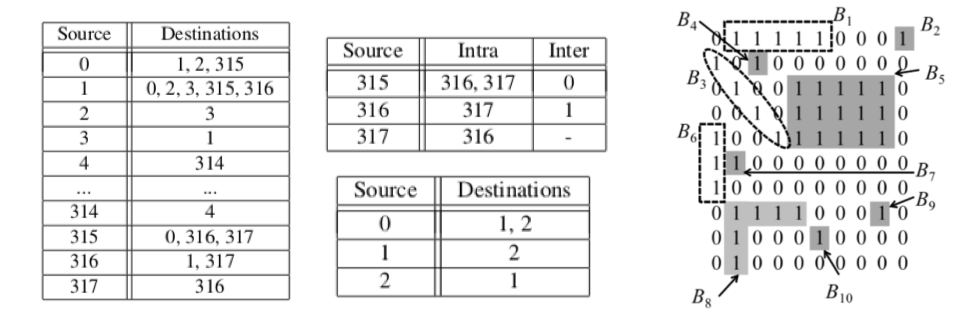
\includegraphics[scale=0.5]{ressources/image/inter_intra.png} 
					\caption{Exemple illustrant le principe de fonctionnement \citep{asano2008efficient}}
					\label{interIntra}
				\end{figure}
							
			Dans une méthode toute récente 
\newacronym{gcupmt}{GCUPMT}{Graph Compression Using Pattern Matching}			
			s'intitulant \gls{gcupmt}, Shah et Rushabh \citep{shah2018graph}  partitionnent les lignes de la matrice d'adjacence en plusieurs blocs ayant la même taille des motifs qui sont dans ce cas sous forme de vecteurs prédéfinies. Les blocs sont comparés avec l'ensemble des motifs ce qui entraîne , en cas de correspondance , le remplacement du bloc par un indicateur du motif précédé par un 1 indiquant que les bits suivants appartiennent à un indicateur de motif. Dans le cas contraire, les données brutes sont stockées directement précédées par un 0.
				
													\begin{landscape}
								\begin{table}
									\begin{tabular}{|c|c|c|c|c|c|c|c|c|c|c|c|c|}
										\hline
										\multirow{2}{*}[-25pt]{Article}  & \multicolumn{4}{c|}{Graphe en entrée} & \multicolumn{2}{c|}{Compression} & \multicolumn{2}{c|}{Structure en sortie}  & \multirow{2}{*}[-25pt]{Graphe de test} & \multirow{2}{*}[-25pt]{Résultat}  \\ \cline{2-11}
				& \rotatebox[origin=c]{90}{ Orienté }  & \rotatebox[origin=c]{90}{ Non orienté } & \rotatebox[origin=c]{90}{ Statique } & \rotatebox[origin=c]{90}{ Dynamique } & \rotatebox[origin=c]{90}{ Avec perte } & \rotatebox[origin=c]{90}{ Sans perte } & \rotatebox[origin=c]{90}{ Succincte } & \rotatebox[origin=c]{90}{ Structurelle }  & & \\ \hline				%%%%%%Fin du header
				
				\hline ECWG
 \citep{asano2008efficient}& \cmark & \cmark & \cmark & \xmark & \xmark &\cmark & \cmark & \xmark  &
										
	\begin{minipage}[t]{0.3\textwidth}
	uk-2002
    \begin{itemize}
    \item 18 millions de nœuds
    \item 298 millions liens\\
    
    \end{itemize}
  \end{minipage}	
										 & 76.1\%	\\
										
										\hline GCUPMT \citep{shah2018graph} & \cmark & \cmark & \cmark & \xmark & \xmark &\cmark & \cmark & \xmark & 
										
	\begin{minipage}[t]{0.3\textwidth}
	graphes avec :
    \begin{itemize}
    \item 8192 nœuds
    \\
    
    \end{itemize}
  \end{minipage}								 
			  & 70\%	\\

										\hline
									\end{tabular}
									\caption{Synthèse des méthode de compression par extraction de motifs basées vocabulaire exploitant les propriétés de la matrice d'adjacence.}									
									
								\end{table}
								
							\end{landscape}
					
				
				%%%%%%%%%%%%%%%%%%%%%%%%%%%%%%%%
				\subsection{Compression basée Agrégation des motifs}
				
					Les méthodes de compression par extraction de motifs basées sur l'agrégation sont des méthodes   qui agrègent plusieurs nœuds ou liens d'un motif en un seul nœud ou lien, appelés respectivement super-nœud et super-lien. Le graphe en sortie, dit super-graphe, devient dès lors plus simple et moins offrant ainsi une aisance et une facilité de traitement, d'exploration et de visualisation. 
					
					Nous présenterons dans ce qui suit les deux sous-classes de cette classe. 
					
					 
					\subsubsection{Compression basée Agrégation de nœuds}
					
					Les techniques de compression basées sur l'agrégation des nœuds des motifs sont des méthodes qui ont existé depuis plusieurs décennies offrant plusieurs avantages. 
					Elles visent à résumer le graphe initial en agrégeant les nœuds des motifs découvert dans le but de diminuer le nombre de nœuds existants  et d'offrir une meilleur visibilité et analyse du graphe. 
						
						Une première méthode de cette classe s'intitulent Subdue \citep{ketkar2005subdue}. Elle effectue une recherche \textit{Branch\&Bound} qui commence à partir de sous-structures composées de tous les sommets avec des étiquettes uniques. Les sous-structures sont prolongées de toutes les manières possibles par un sommet et une arête ou par une arête afin de générer des sous-structures candidates. Subdue conserve les instances de sous-structures et utilise l'isomorphisme de graphe pour déterminer les instances de la sous-structure candidate. Les sous-structures sont ensuite évaluées en fonction de leur compression de la longueur de description (DL) du jeu de données. Cette procédure se répète jusqu'à ce que toutes les sous-structures soient prises en compte ou que les contraintes imposées par l'utilisateur ne soient plus vérifiés. A la fin de la procédure, Subdue indique les meilleures sous-structures de compression.
				Le système Subdue fournit également la possibilité d'utiliser la meilleure sous-structure trouvée lors d'une étape de découverte pour compresser le graphe d'entrée en remplaçant ces instances de la sous-structure par un seul sommet et en effectuant le processus de découverte sur le  compressé. Cette fonctionnalité génère une description hiérarchique du jeu de données de graphe à différents niveaux d'abstraction en termes de sous-structures découvertes.
							
	\citep{rossi2018graphzip} partent de l'observation que les graphes réels sont formés souvent de nombreuses cliques de grande taille. En utilisant ceci comme base, GraphZip décompose le graphe en un ensemble de grandes cliques, qui est ensuite utilisé pour compresser et représenter le graphe de manière succincte. 
												\begin{landscape}
								\begin{table}
									\begin{tabular}{|c|c|c|c|c|c|c|c|c|c|c|c|c|}
										\hline
										\multirow{2}{*}[-25pt]{Article}  & \multicolumn{4}{c|}{Graphe en entrée} & \multicolumn{2}{c|}{Compression} & \multicolumn{2}{c|}{Structure en sortie} & \multicolumn{2}{c|}{Complexité} & \multirow{2}{*}[-25pt]{Graphe de test} & \multirow{2}{*}[-25pt]{Résultat}  \\ \cline{2-11}
				& \rotatebox[origin=c]{90}{ Orienté }  & \rotatebox[origin=c]{90}{ Non orienté } & \rotatebox[origin=c]{90}{ Statique } & \rotatebox[origin=c]{90}{ Dynamique } & \rotatebox[origin=c]{90}{ Avec perte } & \rotatebox[origin=c]{90}{ Sans perte } & \rotatebox[origin=c]{90}{ Succincte } & \rotatebox[origin=c]{90}{ Structurelle } & \rotatebox[origin=c]{90}{ Temporelle} & \rotatebox[origin=c]{90}{ Spaciale} & & \\ \hline				%%%%%%Fin du header
				
				\hline Subdue
 \citep{ketkar2005subdue}& \xmark & \cmark & \cmark & \xmark & \xmark & \cmark & \xmark & \cmark	 & & &		
	\begin{minipage}[t]{0.3\textwidth}
	Composante chimique :
    \begin{itemize}
    \item 21 étiquettes
    \item 422 transactions\\
    
    \end{itemize}
  \end{minipage}	
										 & 16\%	\\
										
										\hline GraphZip \citep{rossi2018graphzip} & \xmark & \cmark & \cmark & \xmark & \xmark & \cmark & \xmark & \cmark & & & 
				Web-Google						
								 
			  & 19\%	\\

										\hline
									\end{tabular}
									\caption{Synthèse des méthodes de compression par extraction de motifs basées agrégation de nœuds.}									
									
								\end{table}
								
							\end{landscape}
						
					\subsubsection{Compression basée agrégation de liens}
						Les méthodes de compression par extraction de motifs basées agrégation de liens sont parmi les méthode les plus populaires. Leur objectif est de produire un graphe compressé à partir du graphe initial en remplaçant les liens denses du graphe par un nouveau super-nœud ou une nouvelle super-arêtes. Elle se divise selon le principe en deux grandes classes: celles utilisant les règles de grammaire et celles utilisant des méthode de clustering. Nous détaillerons dans ce qui suit ces deux classes et nous conclurons par une synthèse sur les méthodes de chaque classe.
						
						 \textbf{Basées sur les règles de grammaire} 
								
								La classe des méthodes de compression basées sur les règles de grammaire est une généralisation d'une méthode de compression des dictionnaire s'intitulant Re-pair. Son principe de base consiste en la  recherche, à chaque itération, de la paire de symboles la plus fréquente dans une séquence de caractères et à la remplacer par un nouveau symbole, jusqu'à ce qu'il ne soit plus commode de les remplacer. Nous notons que dans ce cas le motif est sous forme de deux arêtes ayant un sommet en commun, nommé \textit{digraph}.
								
										Une première méthode de suivant ce principe a été proposée dans \citep{claude2010fast} baptisé \textit{Approximate Re-pair}. Dans cette méthode un graphe G=(V,E) est représenté sous forme d'une sequence de caractères T: \begin{center}
		T=T(G)= $\overline{v_{1}}\ v_{1,1}\ ...\ v_{1,a}\ \overline{v_{2}}\ v_{2,1}\ ...\ v_{2,a_{2}} ... \overline{v_{n}}\ v_{n,1}\ ...\ v_{n,a_{n}}\ $						
\end{center}	
où $\overline{v_{i}}$ représente un indicateur du sommet $v_{i}$. Elle procède en trois étapes essentielles expliquer dans l'algorithme \textbf{\ref{alg:re_pair}} .
	\begin{algorithm}
		\caption{Approximate Re-pair}
		\label{alg:re_pair}
		\begin{algorithmic}[1]
			\STATE \textbf{Calcule des fréquences:} T est parcourue séquentiellement et chaque pair $t_{i}t_{i+1}$ est ajouté à un tableau de hachage H avec leurs nombre d'occurence. 
			\STATE \textbf{Recherche des k meilleurs paires:}  H est parcourue et  les k paires les plus fréquentes sont retenues, en utilisant k pointeurs vers les cellules de H.
			\STATE \textbf{Le remplacement simultané:} les k paires identifiés dans l'étape précédente sont simultanément remplacées par un nouveau identifiant et une règle de production est ajoutée.
		\end{algorithmic}
	\end{algorithm}
	Lorsqu'il n'y a plus de paires à remplacer, Approximate Re-pair s'arrête donnant comme résultat un compressé compacte C de la chaine T. Pour finaliser le processus, tous les indicateurs de nœuds $\overline{v_{i}}$ seront supprimés de C. De plus, l'algorithme crée une table qui contiendra des pointeurs vers le début de la liste d'adjacence de chaque nœud dans C. Grâce à cette table l'algorithme pourra répondre aux requêtes de recherche de successeurs en un temps optimal.
								 %%%%exemple ???
								
	Dans un travail ultérieure \citep{claude2010extended} , les même auteurs s'intéressent aux requêtes de recherche des nœuds prédécesseurs et successeurs à partir du graphe compressé de \textit{Approximate Re-pair} directement. Il proposent alors de combiner leurs méthode avec une représentation basé sur les relations binaires de \citep{barbay2006adaptive}. En effet, ce dernier consiste à représenter les listes d'adjacence à l'aide d'une représentation séquentielle permettant de rechercher les occurrences d'un symbole puis de rechercher les voisins inverses à l'aide de cette primitive. 
								
Claude et Ladra \citep{claude2011practical} partagaient les mêmes préoccupations des auteurs de la méthode précédente et ont proposé comme solution de combiner la méthode Re-pair avec la représentation k2-tree. Ils obtiennent alors une compression de 2,27 (pbe) sur le graphe UK2002, tout en conservant la possibilité d'interroger les voisins entrants et sortants \citep{maneth2015survey}.
							
								
	Une dernière méthode de cette classe s'instituant gRepair a été proposé dans \citep{maneth2018grammar}. Ce nouveau algorithme de compression détecte de manière récursive des sous-structures répétées et les représente via des règles de grammaire.  Des requêtes spécifiques telles que l'accessibilité entre deux nœuds ou des requêtes de chemin normal peuvent ainsi être évaluées en temps linéaire (ou en temps quadratiques, respectivement), sur la grammaire, permettant ainsi des accélérations proportionnelles au taux de compression. la figure xxx presentent le resultat de cette methode sur un exemple. 
								%%%%exemple ???
																						\begin{landscape}
								\begin{table}
									\begin{tabular}{|C{3cm}|c|c|c|c|c|c|c|c|c|c|c|c|}
										\hline
										\multirow{2}{*}[-25pt]{Article}  & \multicolumn{4}{c|}{Graphe en entrée} & \multicolumn{2}{c|}{Compression} & \multicolumn{2}{c|}{Structure en sortie} & \multicolumn{2}{c|}{Complexité} & \multirow{2}{*}[-25pt]{Graphe de test} & \multirow{2}{*}[-25pt]{Résultat (bits/lien)}  \\ \cline{2-11}
				& \rotatebox[origin=c]{90}{ Orienté }  & \rotatebox[origin=c]{90}{ Non orienté } & \rotatebox[origin=c]{90}{ Statique } & \rotatebox[origin=c]{90}{ Dynamique } & \rotatebox[origin=c]{90}{ Avec perte } & \rotatebox[origin=c]{90}{ Sans perte } & \rotatebox[origin=c]{90}{ Succincte } & \rotatebox[origin=c]{90}{ Structurelle } & \rotatebox[origin=c]{90}{ Temporelle} & \rotatebox[origin=c]{90}{ Spaciale} & & \\ \hline				%%%%%%Fin du header
				
				\hline Approximate Re-pair
   \citep{claude2010fast}& \cmark & \xmark & \cmark & \xmark & \xmark &  \cmark & \cmark & \xmark	 & & &		
	\begin{minipage}[t]{0.3\textwidth}
	uk-2002 :
    \begin{itemize}
    \item 18 millions de nœuds
    \item 298 millions de liens\\
    
    \end{itemize}
  \end{minipage}	
										 & 4.23	\\

										\hline Approximate Re-pair \citep{claude2010extended} & \cmark & \xmark & \cmark & \xmark & \xmark & \cmark & \cmark & \xmark  & & & 
										\begin{minipage}[t]{0.3\textwidth}
	uk-2002 :
    \begin{itemize}
    \item 18 millions de nœuds
    \item 298 millions de liens\\
    
    \end{itemize}
  \end{minipage}	 & 3.98 \\ 
  			\hline gRe-pair \citep{maneth2018grammar} & \cmark & \cmark & \cmark & \xmark & \xmark & \cmark & \cmark & \xmark & & &
  				\begin{minipage}[t]{0.3\textwidth}
  			NotreDame :
    \begin{itemize}
    \item 325 milles de nœuds
    \item 1M de liens\\
  		\end{itemize}
  \end{minipage}		
  			& 4.84 \\\hline
									\end{tabular}
									\caption{Synthèse des méthodes de compression par extraction de motifs basées agrégation de liens en utilisant les règles de grammaire.}									
									
								\end{table}
								
							\end{landscape}
								

								
%%% Ajouter son algorithme
%%%% Ajouter un exmple illustant cette methode
								
						 \textbf{Basées sur des méthodes de clustering}
						 
						 		Les méthodes de compression appartenant à la classe courante sont des méthodes basées sur la recherche des sous-graphes denses (ayant des nœuds fortement connectés). Ils sont destinées principalement aux graphes du Web et les graphes des réseaux sociaux dans but de faciliter leurs exploration et analyse.
								
									%-----------------Aggregation des liens ----------%
				\citep{buehrer2008scalable} ont exploité l'existence de plusieurs ensembles de pages web qui ont les même liens sortants. S'intitulant  VNM pour Virtual Node Miner, leurs approche est basée sur la réduction du nombre de liens en créant des nouveaux sommets virtuels qui sont ajoutés au graphe. Soit G = (V,E) un graphe orienté, l'algorithme proposé se compose de deux phases essentielles :
				\begin{enumerate}
				
				
					\item \textbf{Phase de Clustering :}
					
					Le but de cette première étape est de contourner la tâche presque impossible d'extraction simultanée de centaines de millions de points de données en groupant d'abord les sommets similaires dans le graphes dans des clusters. 
				Pour cela k fonctions de hachage indépendantes sont utilisées pour obtenir une matrice de taille V * k. Par la suite, les lignes de la matrice  sont triées lexicographiquement
				%Ce tri est assez rapide car il ne nécessite que O (2V log V) en mémoire à la fois, ce qui tient dans la RAM (ou nous le faisons en minant le graphique en morceaux). 
				et elle est parcourue colonne par colonne en regroupant les lignes ayant la même valeur. Lorsque le nombre total de lignes chute au-dessous d'un seuil ou que le bord de la matrice de hachage est atteint, les identifiants des sommets associés aux lignes sont renvoyé au processus d'extraction (Phase 02). 
					
					\item \textbf{Phase d'Extraction de Motifs :}				Le but de cette étape est de localiser des sous-ensembles communs de liens sortants dans les sommets donnés. 
				Ainsi les ensembles plus grands et fréquents présentent un intérêt, car ils peuvent représenter des motifs plus pertinents et une meilleure compression. En effet, les performances de compression d'un motif  sont calculés en fonction de sa fréquence dans la liste d'adjacence, et de sa taille qui est le nombre de liens qu'il contient \eqref{eqcompperf}.
				%%% Formule
				\begin{equation}
				Compression(P)=(P.fréquence-1)(P.taille-1)-1
				\label{eqcompperf}
				\end{equation}
				Afin d'extraire ces motifs, VNM utilise une heuristique gloutonne. Cette heuristique procède comme suit :
				\begin{enumerate}
				\item Extraire un histogramme des identifiants de liaison sortante à partir de la liste d'adjacence des sommets données.
				\item Les listes sont réorganisées dans l'ordre décroissant des fréquences des liens sortants en éliminant ceux qui apparaissent une seul fois uniquement.
				\item Chaque lien sortant est ajouté à un arbre de préfixes avec l'ensemble trié de ces extrémités initiales selon leurs identifiants. 
				\item L'arbre est par la suite parcouru afin d'identifier les motifs qui maximisent la formule de performance de la compression \ref{eqcompperf}. Ces motifs sont ensuite convertis en nœuds virtuels et les identificateurs de sommet de leurs listes sont supprimés.
				\end{enumerate}
				 
				\end{enumerate}
				
				L'algorithme est appliqué jusqu'à ce que la réduction n'apporte pas un gain significative. La figure \ref{tab:VNM_exm} illustre le principe de fonctionnement de cette méthode sur un exemple.
				
				
			%%%%		Inclure un exemple 
			
		\begin{table}[h!]
			
		 \begin{flushleft}
			\begin{tabular}{C{4cm}||C{9cm} }
				 Phase 01 &  Phase 02 \\
				 {\renewcommand{\arraystretch}{0.6}
					\begin{tabular}[b]{R{0.4cm}|L{0.3cm} L{0.3cm} L{0.3cm}}
				 			id & \(\displaystyle h_{1}\)  & \(\displaystyle h_{2}\) &  \(\displaystyle h_{3}\) \\
							\hline  13 &\cellcolor{blue!25}10&\cellcolor{blue!25}11&\cellcolor{blue!25}12\\
							    	    23 &\cellcolor{blue!25}10&\cellcolor{blue!25}11&\cellcolor{blue!25}12\\
								   	43 &\cellcolor{blue!25}10&\cellcolor{blue!25}11&\cellcolor{blue!25}12\\
				  					55 &\cellcolor{blue!25}10&\cellcolor{blue!25}11&\cellcolor{blue!25}12\\
				  					64 & \cellcolor{blue!25}10&\cellcolor{blue!25}11&\cellcolor{blue!25}12\\
				  					102 &\cellcolor{blue!25}10&\cellcolor{blue!25}11&\cellcolor{blue!25}12\\
				  					204 &\cellcolor{blue!25}10&\cellcolor{blue!25}11&\cellcolor{blue!25}12\\
				  					431 &\cellcolor{blue!25}10&\cellcolor{blue!25}11&\cellcolor{blue!25}12\\
				  					480 &\cellcolor{blue!25}10&\cellcolor{blue!25}11&2\\
				  					501 &\cellcolor{blue!25}10&4&1\\
			\end{tabular}
				
				
				
				1. Calcul des fonctions de hachage et groupement des sommets			
			} &
			{
				 \begin{multicols}{2}
					\renewcommand{\arraystretch}{0.6}
 						 \begin{tabular}{R{0.4cm}|L{3.2cm} }
				 id &  liens sortants \\\hline
				  13 & 1 2 3 8\\
				  23 & 1 2 3 5 6 10 12 15 \\
				  43 & 1 2 3 5 6 10 22 31\\
				  55 & 1 2 3 5 \\
				  64 & 1 2 3 5 6 10 12 15 \\
				  102 & 1 2 3 20\\
				  204 & 1 7 8 9\\
				  431 & 1 2 3 4 5 6 10 22 31\\
			\end{tabular}
			
			
			2.1 la Liste d'adjacence.
			\columnbreak
 				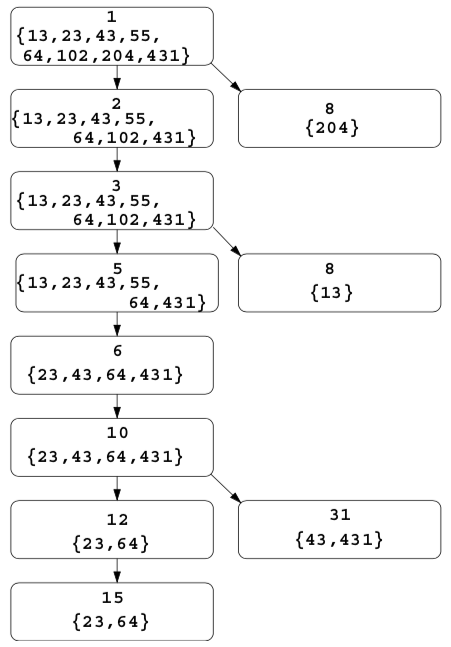
\includegraphics[scale=0.3]{ressources/image/VNM_exemple.png} 
 			%	2.2 Construction de l'arbre
 			
			\end{multicols}
			\begin{center}
		\renewcommand{\arraystretch}{0.6}
		\begin{tabular}{C{1cm} | C{1cm} L{4cm} C{1cm}}
			taille & freq & Liste des noeuds & Savings\\\hline
			6&4&43 431 23 64&14\\
			3&7&23 55 102 64 43 431&11\\
			8&2&23 64&6\\
			7&2&43 431&5\\
		
				\end{tabular}
				2.3 Extraction des Motifs
		\end{center}
			}
			
			\end{tabular}
		\end{flushleft}
		\caption{Exemple d'exécution de VNM}
   			 \label{tab:VNM_exm}
		\end{table}
		
		%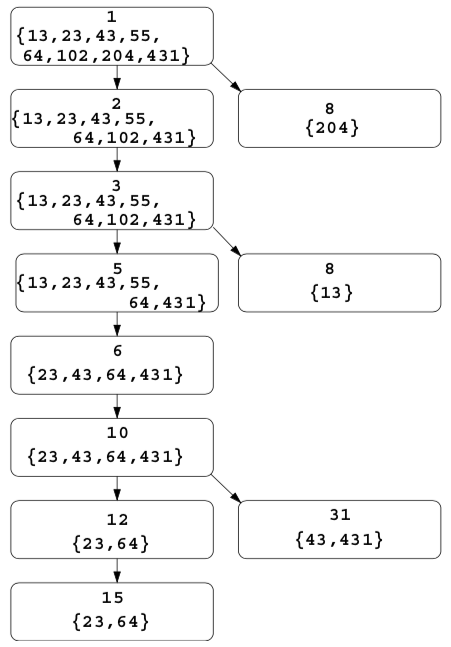
\includegraphics[scale=0.5]{ressources/image/VNM_exemple.png}
									Une variante de VNM a été proposée par Hernandez et Navarro \citep{hernandez2014compressed}. Comme première contribution, ils augmentent les types de structures découvertes dans la phase de clustering pour englober aussi: les cliques, les bi-cliques. L'extraction de motifs cette fois-ci n'est basée sur un parcours des feuilles vers la racine mais l'inverse où  l'ensemble des sommets finales des liens du motifs est constitués des étiquettes des nœuds de l'arbre inclus dans le chemin de la racine vers la feuille et  les sommets initiales sont la liste des sommets inclus dans le nœud feuille. 
				%%Noublie pas revient vers la source 
				Leurs deuxième contribution consiste en une hybridation dans le but de représenter le graphe en sortie à l'aide de structures compactes. Une première approche proposée est d'utiliser les  k2-trees \citep{brisaboa2009k} et qui donnent la représentation la plus compacte.  
				La deuxième hybridation consiste en une nouvelle structure proposée par les auteur.\\
				%revoire cela avec SAnna
				\begin{figure}[h]
					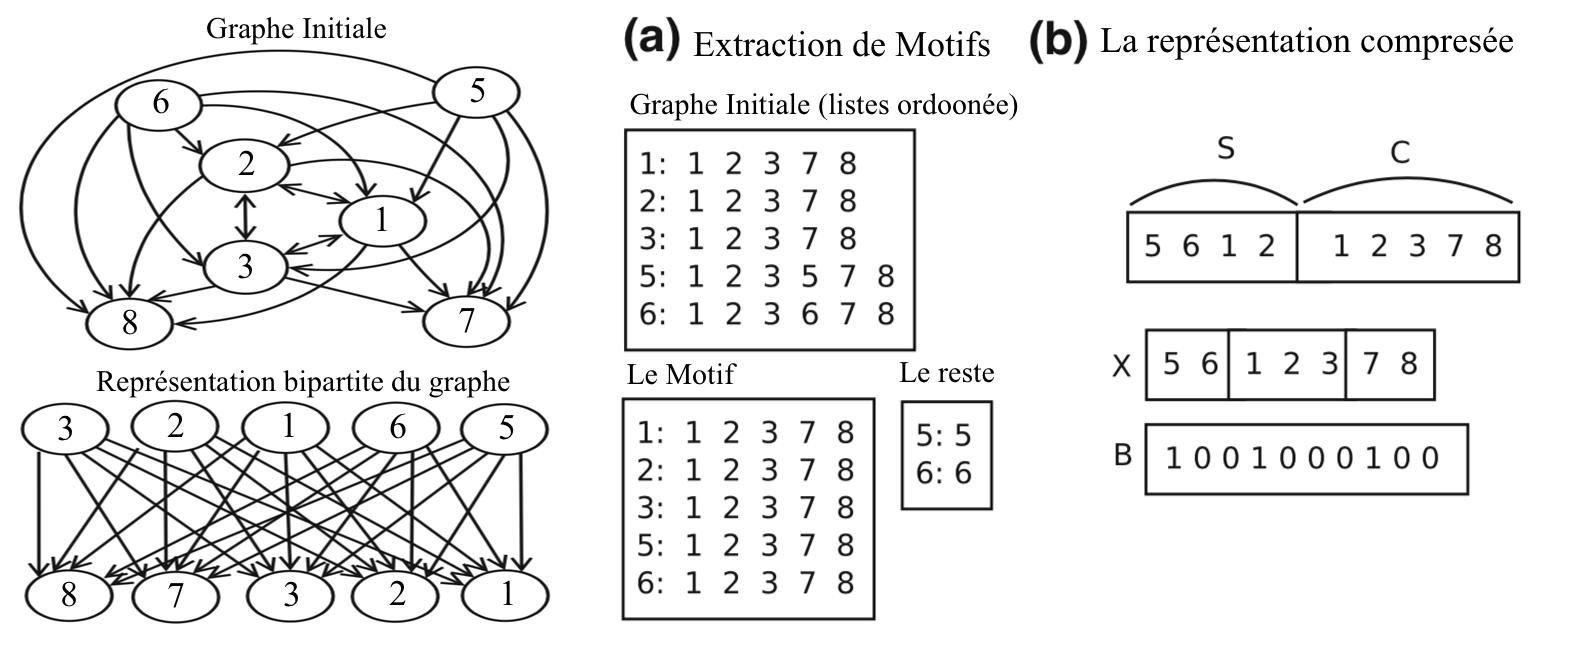
\includegraphics[scale=0.25]{ressources/image/VNM2_exemple.png} 
					\caption{Exemple d'exécution de SDM}
					\label{SDM}
				\end{figure}
										\begin{landscape}
								\begin{table}
									\begin{tabular}{|C{4cm}|c|c|c|c|c|c|c|c|c|c|c|c|}
										\hline
										\multirow{2}{*}[-25pt]{Article}  & \multicolumn{4}{c|}{Graphe en entrée} & \multicolumn{2}{c|}{Compression} & \multicolumn{2}{c|}{Structure en sortie}  & \multirow{2}{*}[-25pt]{Graphe de test} & \multirow{2}{*}[-25pt]{Résultat (bits/lien)}  \\ \cline{2-11}
				& \rotatebox[origin=c]{90}{ Orienté }  & \rotatebox[origin=c]{90}{ Non orienté } & \rotatebox[origin=c]{90}{ Statique } & \rotatebox[origin=c]{90}{ Dynamique } & \rotatebox[origin=c]{90}{ Avec perte } & \rotatebox[origin=c]{90}{ Sans perte } & \rotatebox[origin=c]{90}{ Succincte } & \rotatebox[origin=c]{90}{ Structurelle } & & \\ \hline				%%%%%%Fin du header
				
				\hline VNM
 \citep{buehrer2008scalable}& \cmark & \xmark & \cmark & \xmark & \xmark & \cmark & \xmark & \cmark &		
	\begin{minipage}[t]{0.3\textwidth}
	uk-2002 :
    \begin{itemize}
    \item 18 millions de noeuds
    \item 298 millions de liens \\
    
    \end{itemize}
  \end{minipage}	
										 & 1.95\	\\
										
										\hline DSM \citep{hernandez2014compressed} & \cmark & \xmark & \cmark & \xmark &  \xmark & \cmark & \cmark & \cmark  & 
				\begin{minipage}[t]{0.3\textwidth}
	uk-2002 :
    \begin{itemize}
    \item 18 millions de noeuds
    \item 298 millions de liens \\
    
    \end{itemize}
  \end{minipage}						
								 
			  & 1.53	\\

										\hline
									\end{tabular}
									\caption{Synthèse des méthodes de compression par extraction de motifs basées agrégation de liens en utilisant des heuristiques de clustering.}									
									
								\end{table}
								
							\end{landscape}
						
												
								
		\section{Conclusion}


%---->chapitre 03 :« Etude empirique »
	\chapter{Contribution}
		%%%%
		\section{Formulation du problème}
			\subsection{Description conceptuelle}
			\subsection{Pseudo algorithme}
		\section{Analyse de complexité}
		\section{Conclusion}
	
	
	
	
	%\begin{defn}
	%		Here is a new definition
	%\end{defn}
	

%Conclusion Générale									Obligatoire
\chapter{Conclusion} 

%Références Bibliographiques (fin de la pagination)		Obligatoire

%Annexes													Selon besoin


\newpage
\bibliography{Bibliographie}
\bibliographystyle{apalike}

\end{document}

%\renewcommand{\thefigure}{\arabic{figure}}
%\setcounter{figure}{0}
%\begin{figure}[H]
%	\centering
%	\includegraphics[scale=1]{ressources/image/LAAS-2016.jpg}
%	\label{fig:figure1}
%	\caption{This is a teste of figure}
	
%\end{figure}








